\chapter{Analytical Model}
\label{ch:analyticalmodel}
%\textit{This chapter presents a calculation of the critical current in a SNS junctions. For this purpose, a quasiclassical transport theory is used and its foundations are explained in the first section. This technique is then employed for a clean SNS junction, and an expression for the Josephson current is found. In the following section, the calculations used for the clean setup are extended for the more sophisticated quantum point contact (QPC) and here as well, the current for the QPC-gated junction is found.}

\section{Foundation Of The Quasi-classical Model}
%This section explains preliminary assumptions made to describe the current in a SNS junction. 
From section \ref{sec:theory-sns} it is known that Andreev reflection of electrons in a SNS junction leads to Andreev bound states within the junction. Each one of these bound states contributes to the total current through the junction. Essentially, a bound state can be expressed as a trajectory from one superconductor through the normal metal to the other superconductor. The superconducting current density is found through geometrical analysis of possible trajectories. The total current density is then found by adding up all these trajectories.
%The superconducting current density is found by summing up these trajectories. This is a way to express the current through geometrical analysis of possible trajectories only. The underlying material does not play a specific role in the calculation, which makes this approach universally applicable.
\begin{figure}[h]
\centering	
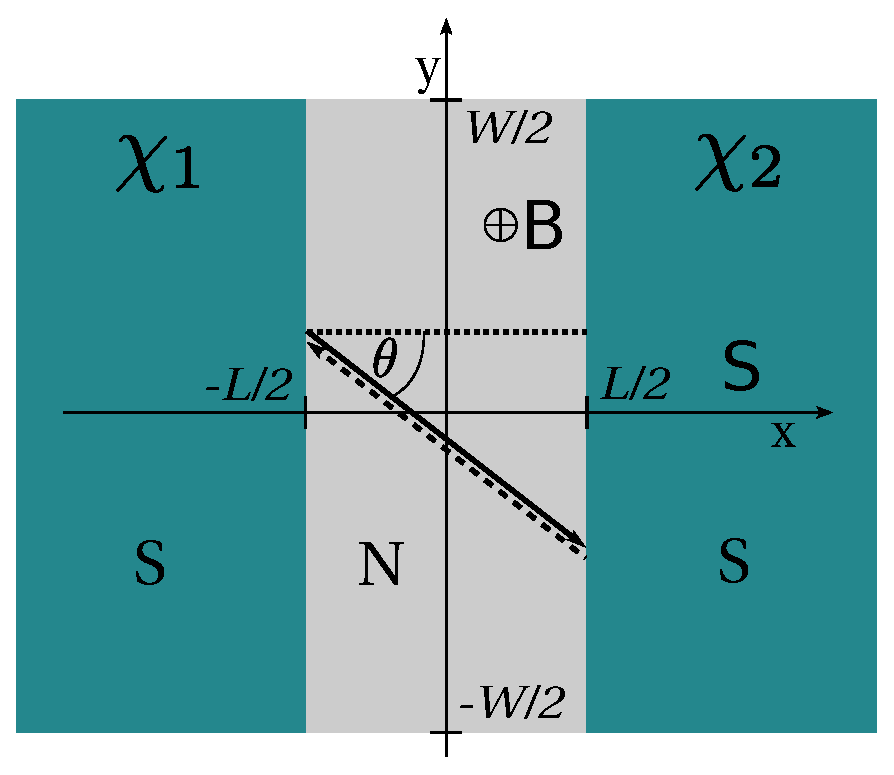
\includegraphics[width=0.6\textwidth]{figure/analyticalmodel/sns_junction_csch}
\caption{An SNS junction with width $W$ and length $L$. A trajectory connecting the interfaces is parametrized by the angle $\theta$ between the trajectory and the x-axis. $\chi_1$ and $\chi_2$ are the superconducting phases, with total phase difference $\chi = \chi_2 - \chi_1$.}
\label{fig:sns_schematic}
\end{figure}
The two dimensional junction (schematic shown in fig \ref{fig:sns_schematic}) is a short and wide junction with width $W$ and length $L$, where $W \gg L$. The NS-interfaces are parallel to the $y$-axis and are placed at $x = \pm L/2$. Each of the superconducting leads has a phase $\chi_{1}$ and $\chi_{2}$, and the overall phase difference is $\chi = \chi_{1} - \chi_{2}$. The superconducting gap parameter $\Delta$ is only present in the superconducting leads. Close to the interface, $\Delta$ begins to decay on a length scale of the superconducting coherence length $\xi_0$ into the normal region.
%\begin{equation}
%\xi_0 = \hbar v_F / \pi \Delta.
%\end{equation} 
Similar to the procedure in section \ref{sec:theory-sns}, this decay is neglected and a step-like behaviour is assumed for the superconducting gap parameter:
\begin{equation}
\Delta\left( x \right) = |\Delta| e^{\chi_1} \Theta\left(-L/2 -x \right) + |\Delta| e^{\chi_2} \Theta\left(x-L/2 \right).
\label{eq:gap_parameter}
\end{equation}
The thermal length scale of the system assumed to be larger than the sample length:
\begin{equation}
L_T = \hbar v_F / k_B T \gg L.
\end{equation}
The transport through the junction is assumed to be ballistic, resulting in the trajectories being straight and not being altered by scattering in the normal region. However, the presence of the magnetic field in the normal region of the sample will lead to a bending of the trajectories due to the Lorentz force. Depending on the strength of magnetic field $B$ and the Fermi velocity, the radius of this curve is 
\begin{equation}
r_B = \frac{m v_F}{e B}
\end{equation}
In order to justify the assumption of straight trajectories, either the magnetic field has to be weak enough, or the Fermi velocity (wavelength) has to be large (short) enough. Then, the cyclotron radius $r_B$ is larger than the sample size $L$, and straight trajectories are a valid assumption. 

\section{Plane Set-up: Calculation Of The Critical Current}
Summing up the contributions leads to the current through the SNS junctions, the Josephson current $J\left( \chi \right)$, which is a function of the superconducting phase difference $\chi = \chi_2 - \chi_1$. By maximizing the Josephson current with respect to $\chi$, one finds the critical current $I_c$.\\
A trajectory connecting the two superconducting interfaces can be parametrized by the angle $\theta$ between the trajectory and the x-axis. For a trajectory from a point $(-L/2, y_1)$ to another at $(+L/2, y_2)$, the angle for the parametrization is
\begin{equation}
\tan \theta = \frac{y_2 - y_1}{L}.
\label{eq:parametrization}
\end{equation}
Figure \ref{fig:sns_schematic} visualizes this parametrization. 
Several papers outline approaches to this problem (\cite{Zagoskin1997}, \cite{Barzykin1999}) and are based on the same concept. The Josephson current in \cite{Zagoskin1997} has the form
\begin{equation}
J =  \frac{2 e }{\pi L} \sum_{\bm{\kappa}}v^{\bm{\kappa}}_{Fx} \mathcal{J} \left(\chi\right), \label{eq:i-zagoskin}
\end{equation}
where $\bm{\kappa}$ is the tangential momentum with $\bm{\kappa}^2 + \mathbf{k_x}^2 = k_F^2$.
%TODO simply \kappa = k_y?
$v_{Fx}$ is the projection of $v_F$ on the x-axis
\begin{equation}
v_{Fx} =  v_F  \cos \theta
\end{equation}
and $\mathcal{J} \left( \chi \right)$ is the current density. A similar ansatz to eq. (\ref{eq:i-zagoskin}) is described in \cite{Meier2016}:
\begin{equation}
J =  \int_{-W/2}^{+W/2} dy \int_{-p_F}^{+p_F} \frac{dp_y}{2 \pi} \cos \theta \mathcal{J} \left( \chi, \phi \right).
\end{equation}
For a fixed point at the left interface, the current density is integrated over all possible momenta. This integral can be expressed through the endpoints of a trajectory. The integration over $p_y$ can then be replaced by $p_y = p_F \sin \theta \rightarrow d p_y/d\theta = p_F \cos \theta$. The integration over the angle $\theta$ can be substituted by the integration over $y_2$, a point at the right interface. The result for the Josephson current reads
\begin{equation}
J\left(\chi, \phi=0\right) = \frac{2 e v_F}{\pi \lambda_F L^2}  \int \int_{-W/2}^{W/2} d y_1 d y_2 \frac{\mathcal{J}(\chi)}{\left[ 1 + \left(\frac{y_1 - y_2}{L}\right)^2\right]^2}.
\label{eq:josephson_current_zero_b}
\end{equation}
By maximizing the Josephson current with respect to $\chi$, the critical current can be found as:
\begin{equation}
I_c(\phi) = \text{max}_{\chi}\left\{ J(\chi, \phi) \right\}\label{eq:josephson-relation}.
\end{equation}
%TODO insert result of integration with B=0
The current density $\mathcal{J}$ depends on the ratio of $W$ and $L$. For $W \gg L$, the junction is a short junction, while for $W \ll L$, it is a long junction. 
In the short junction limit, the current density is calculated in \cite{Beenakker1991}
\begin{equation}
\mathcal{J}^s (\chi) = \frac{\mathcal{T}_n \sin \chi}{\sqrt{1 - \mathcal{T}_n \sin^2 \frac{\chi}{2}}}\label{eq:short-j}
\end{equation}
which can be derived in the framework of the scattering matrix formalism. $\mathcal{T}_n$ is the transmission coefficient for a given conducting channel. For low transmission, $\mathcal{T} \ll 1$, only the first addend contributes, which leads to the conventional Josephson relation $J \simeq \mathcal{T} \sin \chi$.\\
For the long junction, from \cite{Barzykin1999} the following expression can be found:
\begin{equation}
\mathcal{J}^l(\chi) = \sum_{k = 1}^{\infty} \frac{(-1)^{k+1} \mathcal{T}^k}{k} \sin( k \chi).\label{eq:long-j}
\end{equation}
The coefficient $\mathcal{T}$ has been included phenomenologically in this formula and includes the normal scattering in the sample.
\begin{figure}
\centering
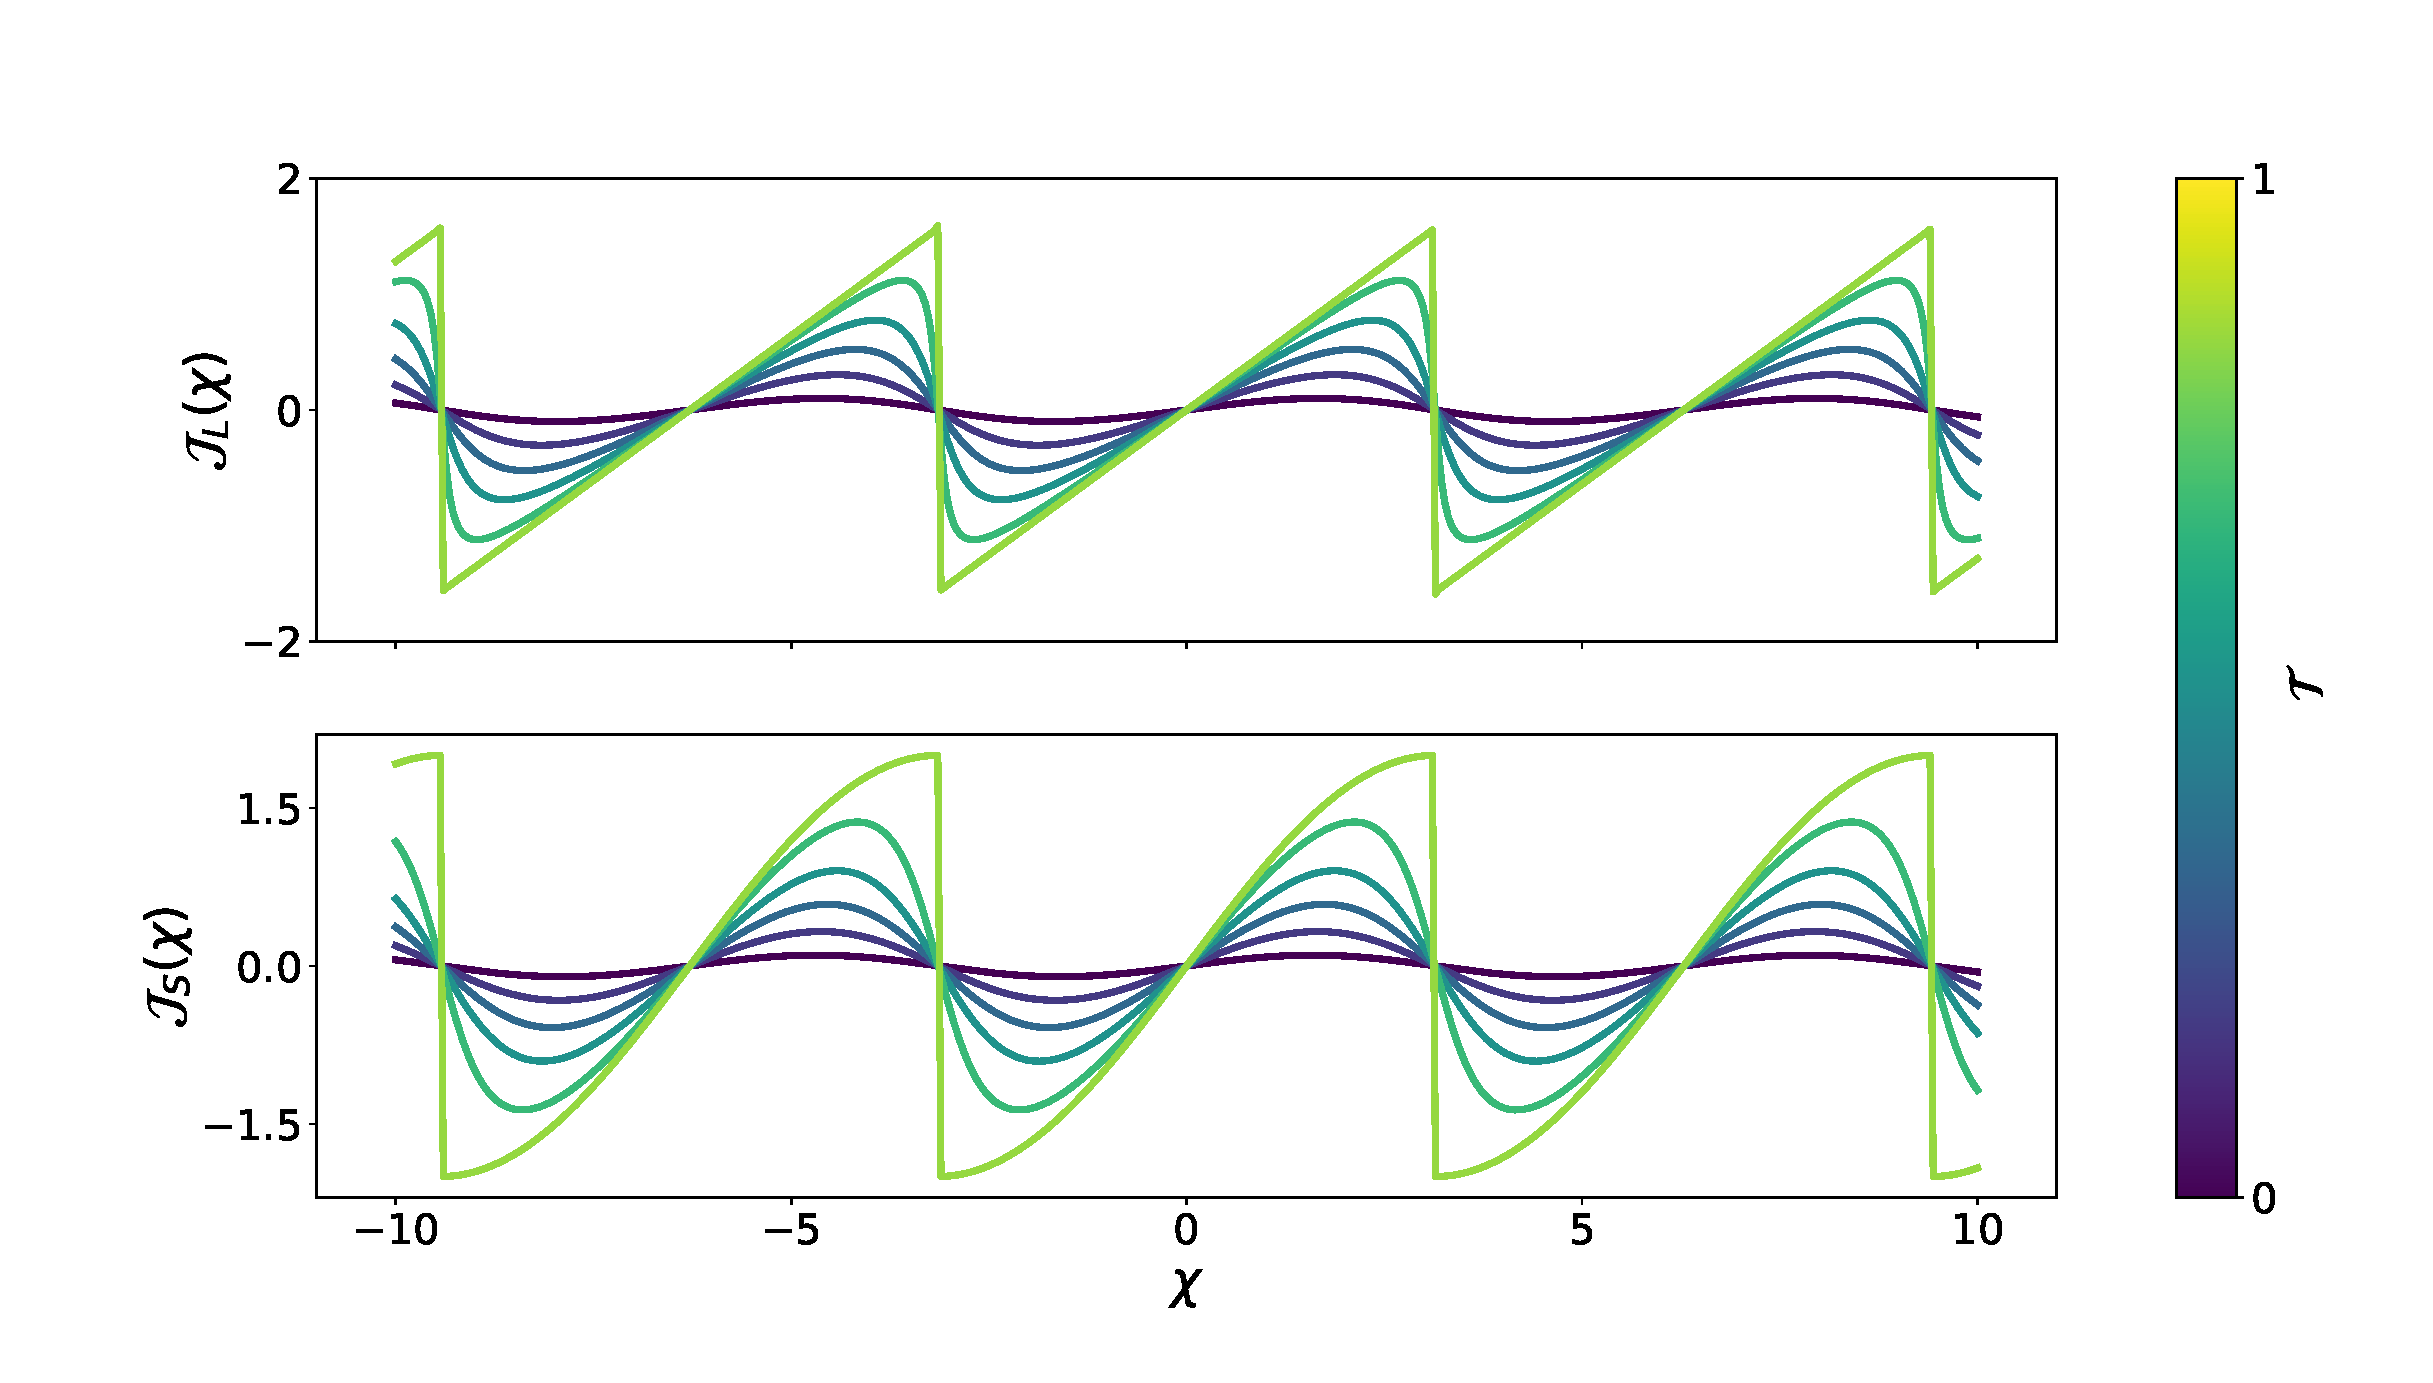
\includegraphics[width=\textwidth]{figure/analyticalmodel/current_density_all}
\caption{Current density plotted against the superconducting phase difference $\chi = \chi_2 - \chi_1$. The density from eq. (\ref{eq:long-j}) gives the sawtooth like shape for $\mathcal{J}^l$ for high values of $\mathcal{T}$. In the short junction limit, $\mathcal{J}^s$ holds from eq. (\ref{eq:short-j}). For low values of the transmission coefficient $\mathcal{T}$, both current densities have a similar sinusoidal form. }
\label{fig:current_density}
\end{figure}
Figure \ref{fig:current_density} shows a plot of both short and long junction limit current densities. For $\mathcal{T} \ll 1$, $\mathcal{J}^s$ takes a sinusoidal form, which also true for the long junction limit. For each of those, the classical Josephson relation can be found in the limit of low transmissions:
\begin{equation}
\mathcal{J} \simeq \mathcal{T} \sin \chi \label{eq:josephson-low-t}
\end{equation} The current densities differ for a large transmission coefficient $\mathcal{T} \simeq 1$: A sawtooth-like shape is observed in the long junction limit, and in the short junction limit, a sinusoidal shape appears.\\

%%%%%
\subsection*{Including Magnetic Field}
Up to this point, the current has been derived for zero magnetic field. If a finite magnetic field is considered, the phase $\chi$ is modified because of two effects: First, the magnetic phase that will be acquired along a trajectory connecting two points $y_1$ and $y_2$  leads to an additional term in the phase. Also, the superconducting phases at each interface become functions of $y_{1/2}$ (see \cite{Meier2016}):
%Then again, \textit{the condition of zero screening current in the bulk superconducting region and the limit of} $\lambda_L \rightarrow 0$ \textit{require the superconducting phase at the interfaces to become functions of y.
\begin{eqnarray}
\chi_{1/2} &=& \mp \frac{1}{2}\left( \chi - \frac{2 \pi B L }{\phi_0} y_{1/2}\right) \\
\tilde{\chi}(y_1, y_2) &=& \chi_2 - \chi_1 \\
 &=& \chi - \frac{\pi B L}{\phi_0}(y_1 + y_2)
 \label{eq:chi}
\end{eqnarray}
Assuming that the London penetration depth is small to zero in the superconducting regions, the following gauge for the vector potential can be used:
\begin{equation}
\mathbf{A}=A_y \mathbf{e}_y, \quad
A_y=\left\{ 
		\begin{array}{ll}
				-B x, & -L/2 \leq x \leq L/2, \\[0.2cm] 
				-\frac{1}{2} B L |x| , & \quad |x|>L/2
		\end{array} 
	\right.
\label{eq:Ay}
\end{equation}
This gauge will give no additional contribution to the phase on straight trajectories
\begin{eqnarray}
\delta \chi &=& \frac{2 \pi}{\Phi_0} \int d \mathbf{l} \cdot \mathbf{A} \\
&=& \frac{2 \pi}{\Phi_0} \int_{-L/2}^{L/2} \frac{dx}{\cos \theta} A_y (x) \sin \theta \\
&=& - \frac{2 \pi B}{\Phi_0} \frac{y_2 - y_1}{L} \int_{-L/2}^{L/2} x dx \\
&=& 0, \label{eq:magnetic-phase-straight}
\end{eqnarray}
where eq.~(\ref{eq:parametrization}) has been used. The total phase for this setup is therefore eq.~(\ref{eq:chi}). This results in the current phase relation in the expression for the Josephson current from eq. (\ref{eq:josephson_current_zero_b}) to be replaced by the effective phase $\chi \rightarrow \tilde{\chi}(y_1, y_2)$:
\begin{equation}
J\left(\chi, \phi \right) = \frac{2 e v_F}{\pi \lambda_F L^2}  \int \int_{-W/2}^{W/2} d y_1 d y_2 \frac{\mathcal{J}(\tilde{\chi}(y_1, y_2))}{\left[ 1 + \left(\frac{y_1 - y_2}{L}\right)^2\right]^2}
\end{equation}
Here, the expression for the supercurrent density in the long junction limit and in the limit of low transmission, eq. (\ref{eq:josephson-low-t}) is used. Plugging in the effective phase from eq.~(\ref{eq:chi}), the Josephson current reads
\begin{equation}
J(\tilde{\chi}(y_1, y_2), \phi) = \mathcal{T}  \sin \chi  \frac{2 e v_F}{\pi \lambda_F L^2} \int \int_{-W/2}^{W/2} d y_1 d y_2 \frac{\cos \left( \frac{\pi \phi}{W}(y_1 + y_2) \right)}{\left[ 1 + \left(\frac{y_1 - y_2}{L}\right)^2\right]^2} \label{eq:josephson_current},
\end{equation}
where $\sin \tilde{\chi}$ has been rearranged in term of trigonometric functions. Since the integration is symmteric in the limits, only the term with $\cos ( \frac{\pi \phi}{W}(y_1 + y_2) )$ is being kept in the expression for the current. Maximizing the Josephson current with respect to $\chi$ gives $\sin\chi \rightarrow 1$. 

The result for the critical current at zero temperature for the limits of a wide and narrow junction has been done in\cite{Barzykin1999} and is found
\begin{eqnarray}
I_c(\nu) &=& \frac{2 e v_F }{\lambda_F L^2}\frac{( 1- \{ \nu \}) \{ \nu \} }{|\nu|}, \quad W/L \gg 1 \label{eq:ic-short}\\
I_c(\nu) &=& \frac{e v_F }{\lambda_F L^2}\frac{( 1- \{ \nu/2  \})^2 \{ \nu/2 \}^2 }{|\nu/2|^2}, \quad W/L \ll 1 \label{eq:ic-long}
\end{eqnarray}
where $\nu = \phi / \phi_0 $ and $\mathcal{T} \approx 1$. The fractional part of $\nu$ is denoted with $\{ \nu \}$. Depending on the geometry of the sample, in particular depending on the raio $W/L$, the periodicity of the Fraunhofer pattern changes. For a wide junction ($W/L \gg 1$), the critical curve is periodic in $phi_0$. With a changing ratio, the periodicity changes. In the other limit of a narrow junction with  $W/L \ll 1$, the Fraunhofer pattern has a $2\phi_0$ periodicity.
\begin{figure}
\centering
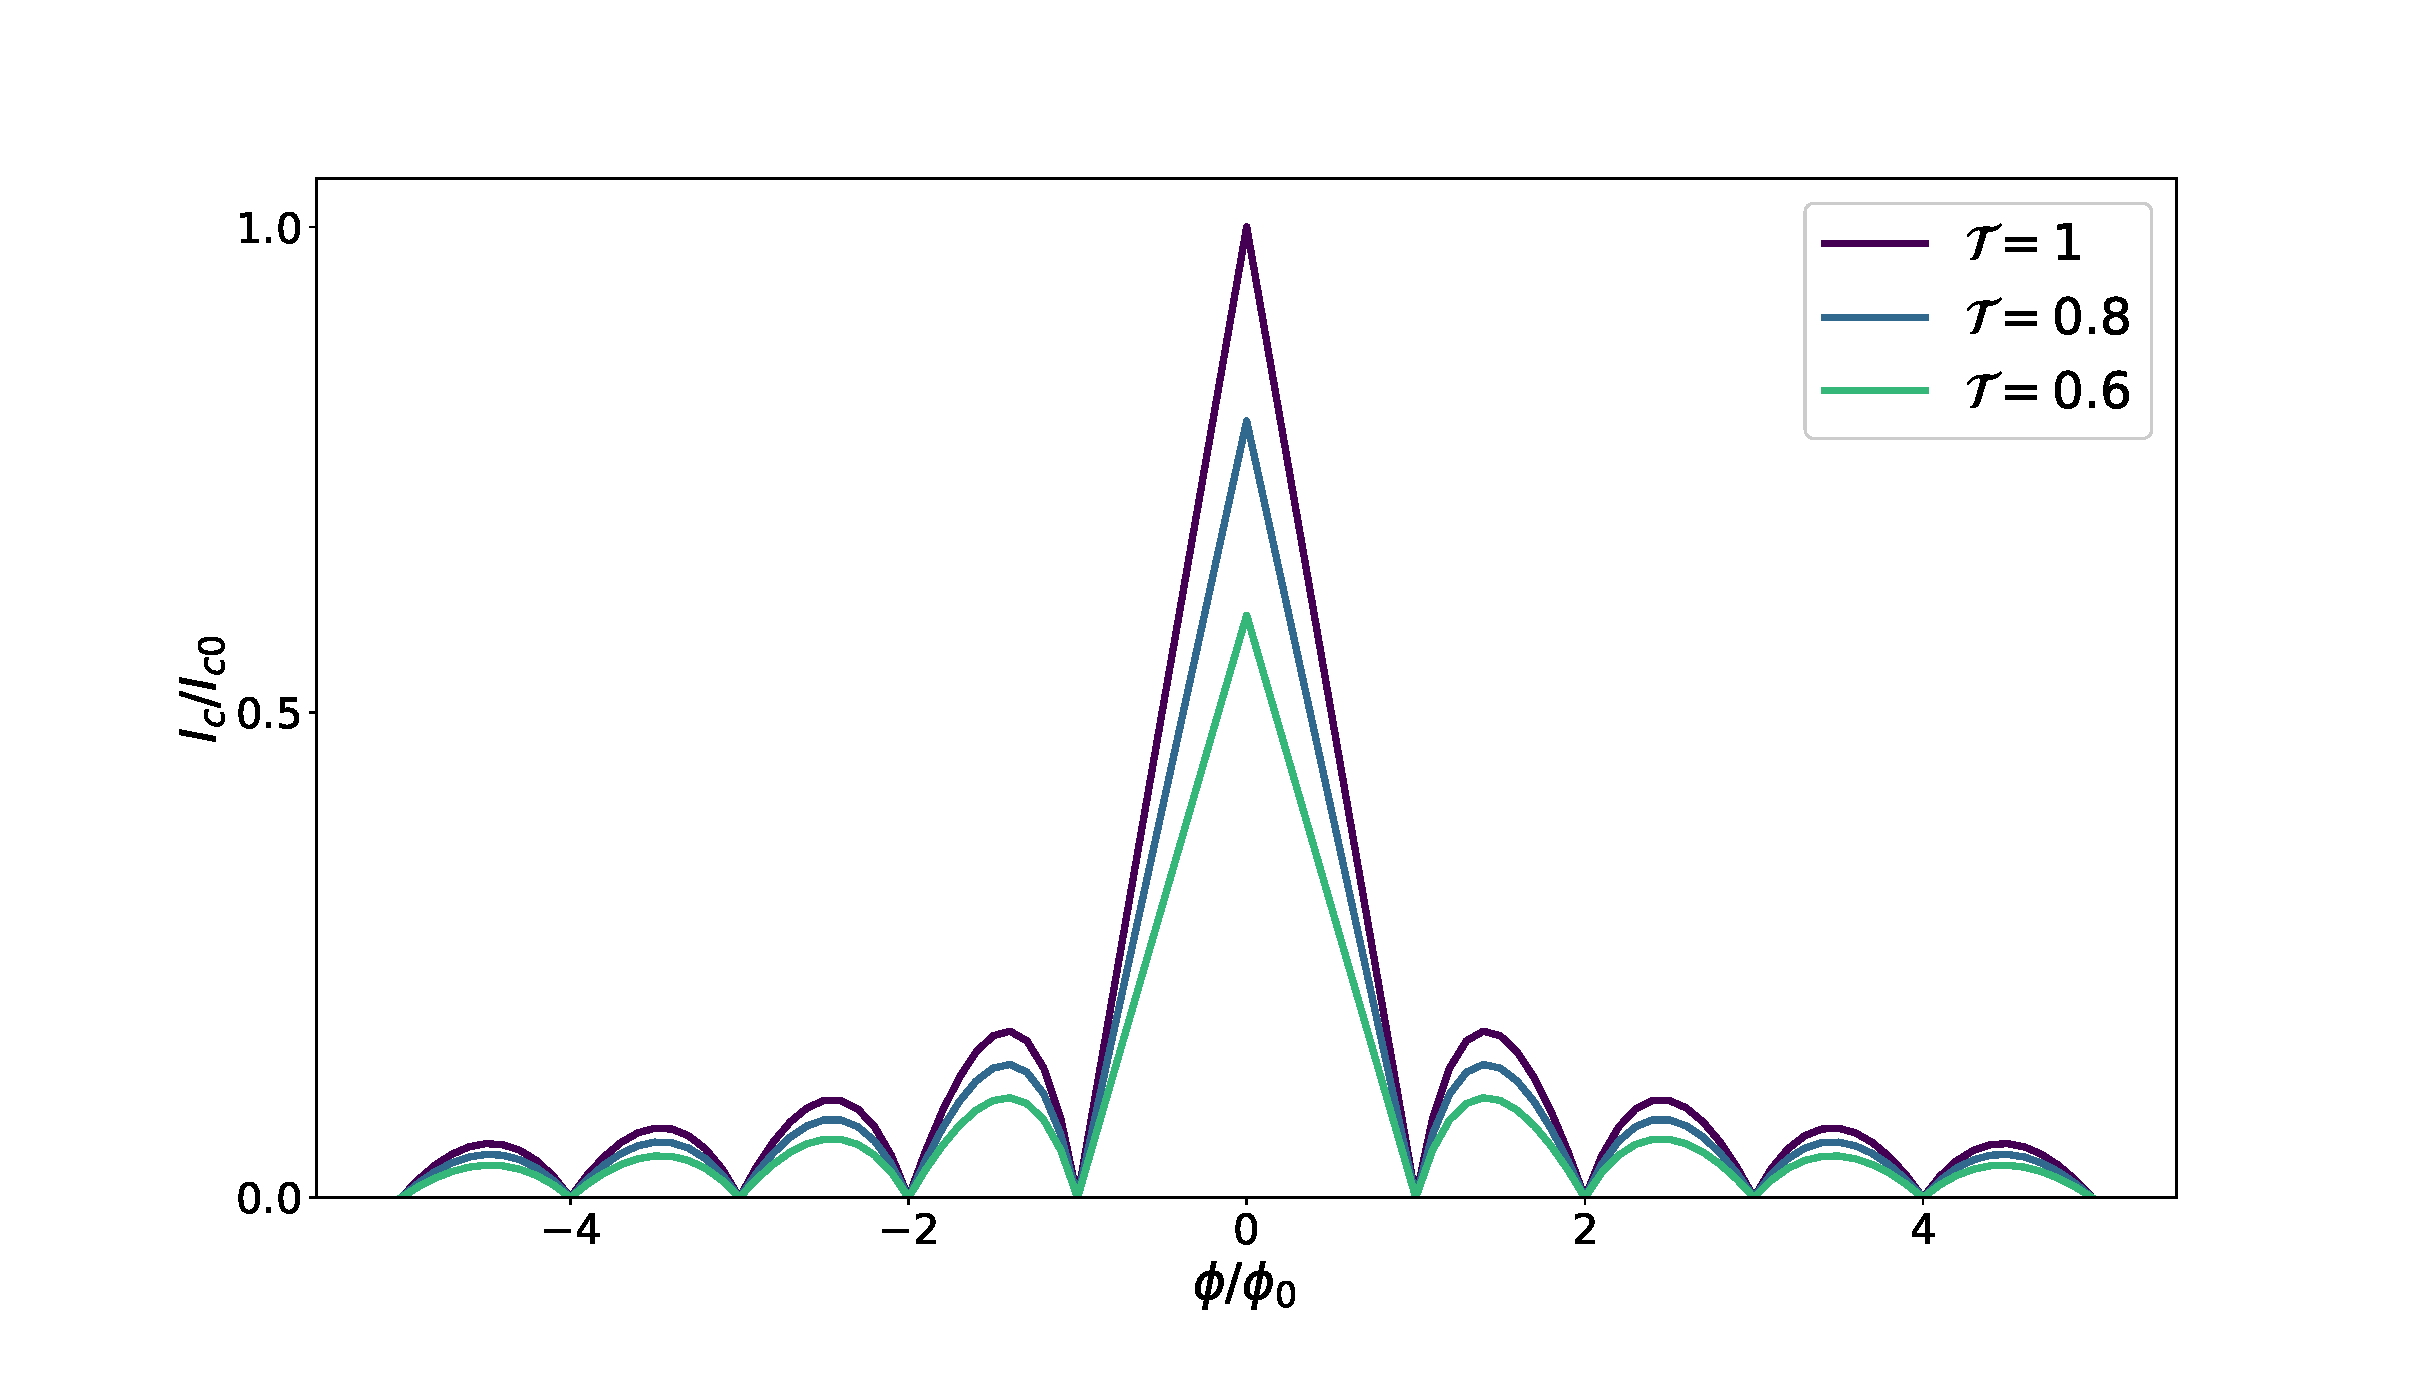
\includegraphics[width=0.8\textwidth]{figure/analyticalmodel/ic_vs_tau}
\caption{The normed critical current $I_c/I_0$ versus $\phi / \phi_0$ for different transmissions cofficients $\mathcal{T}$. For $\mathcal{T} > 1$, the barrier becomes reflective and the overall current density is low. The sharp peak ar $\phi / \phi_0$ arises from the  }
\end{figure}
\begin{figure}
\centering
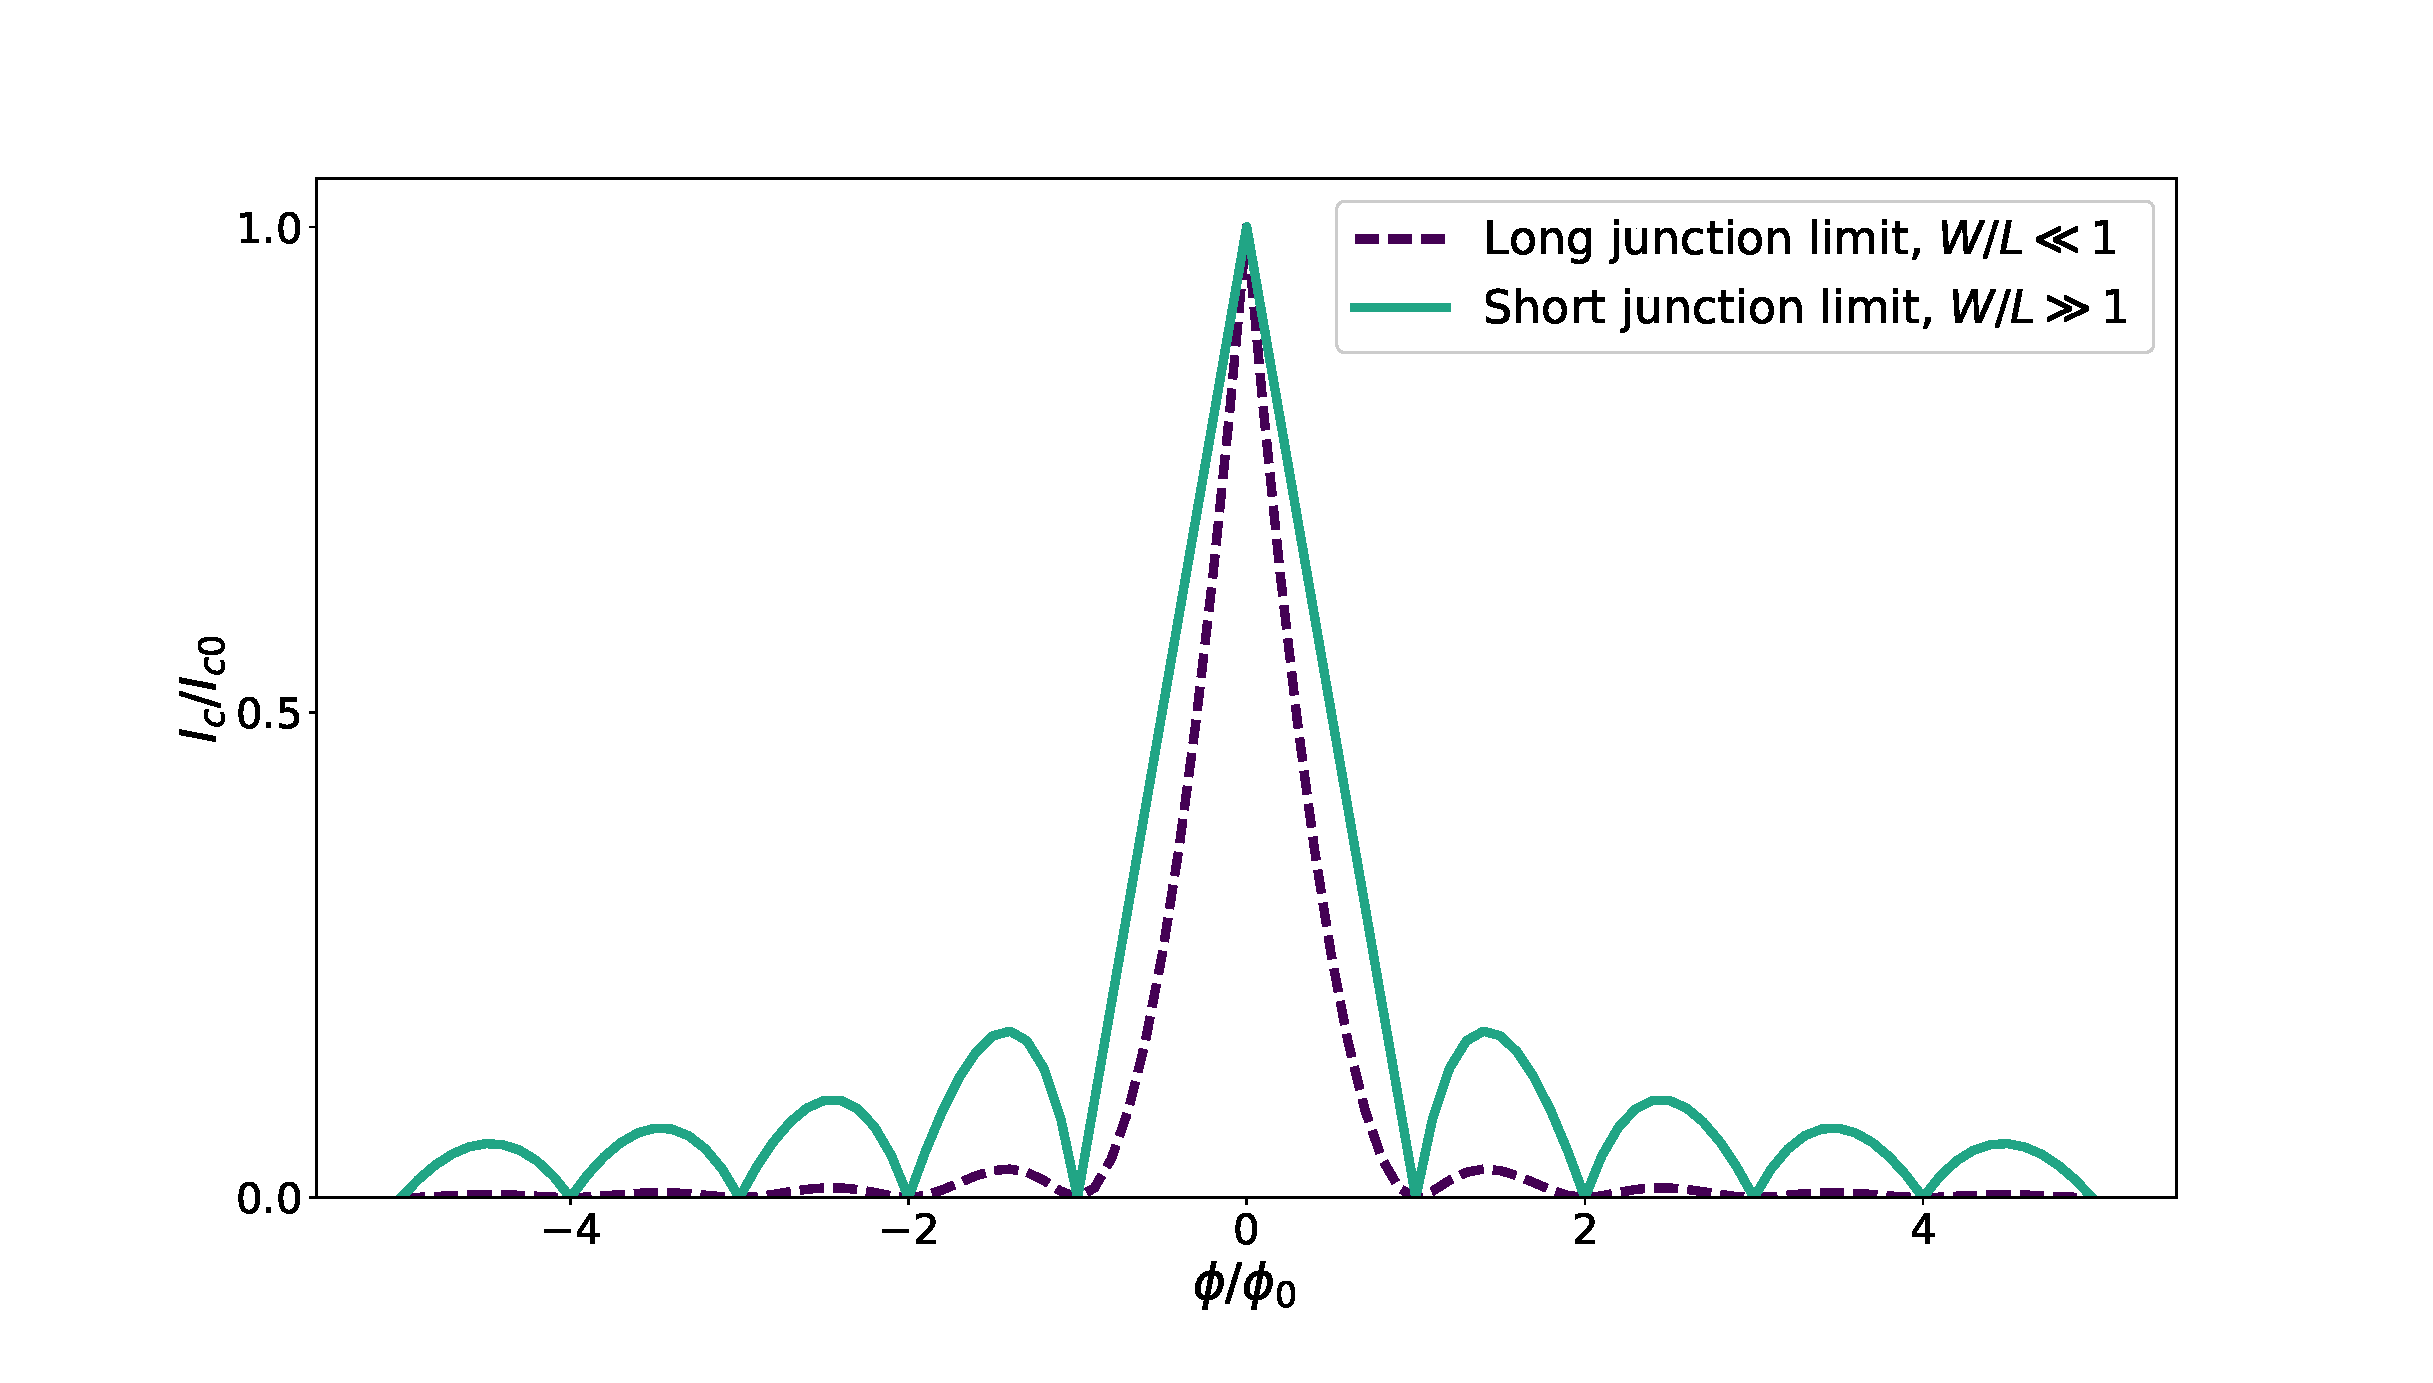
\includegraphics[width=0.8\textwidth]{figure/analyticalmodel/ic-long-vs-short}
\caption{Normed critical current calculated from eqs. (\ref{eq:ic-long}) and (\ref{eq:ic-short}) for the long and short junction limit, respectively. }
\end{figure}

%\begin{figure}
%\centering
%\begin{minipage}{0.5\textwidth}
%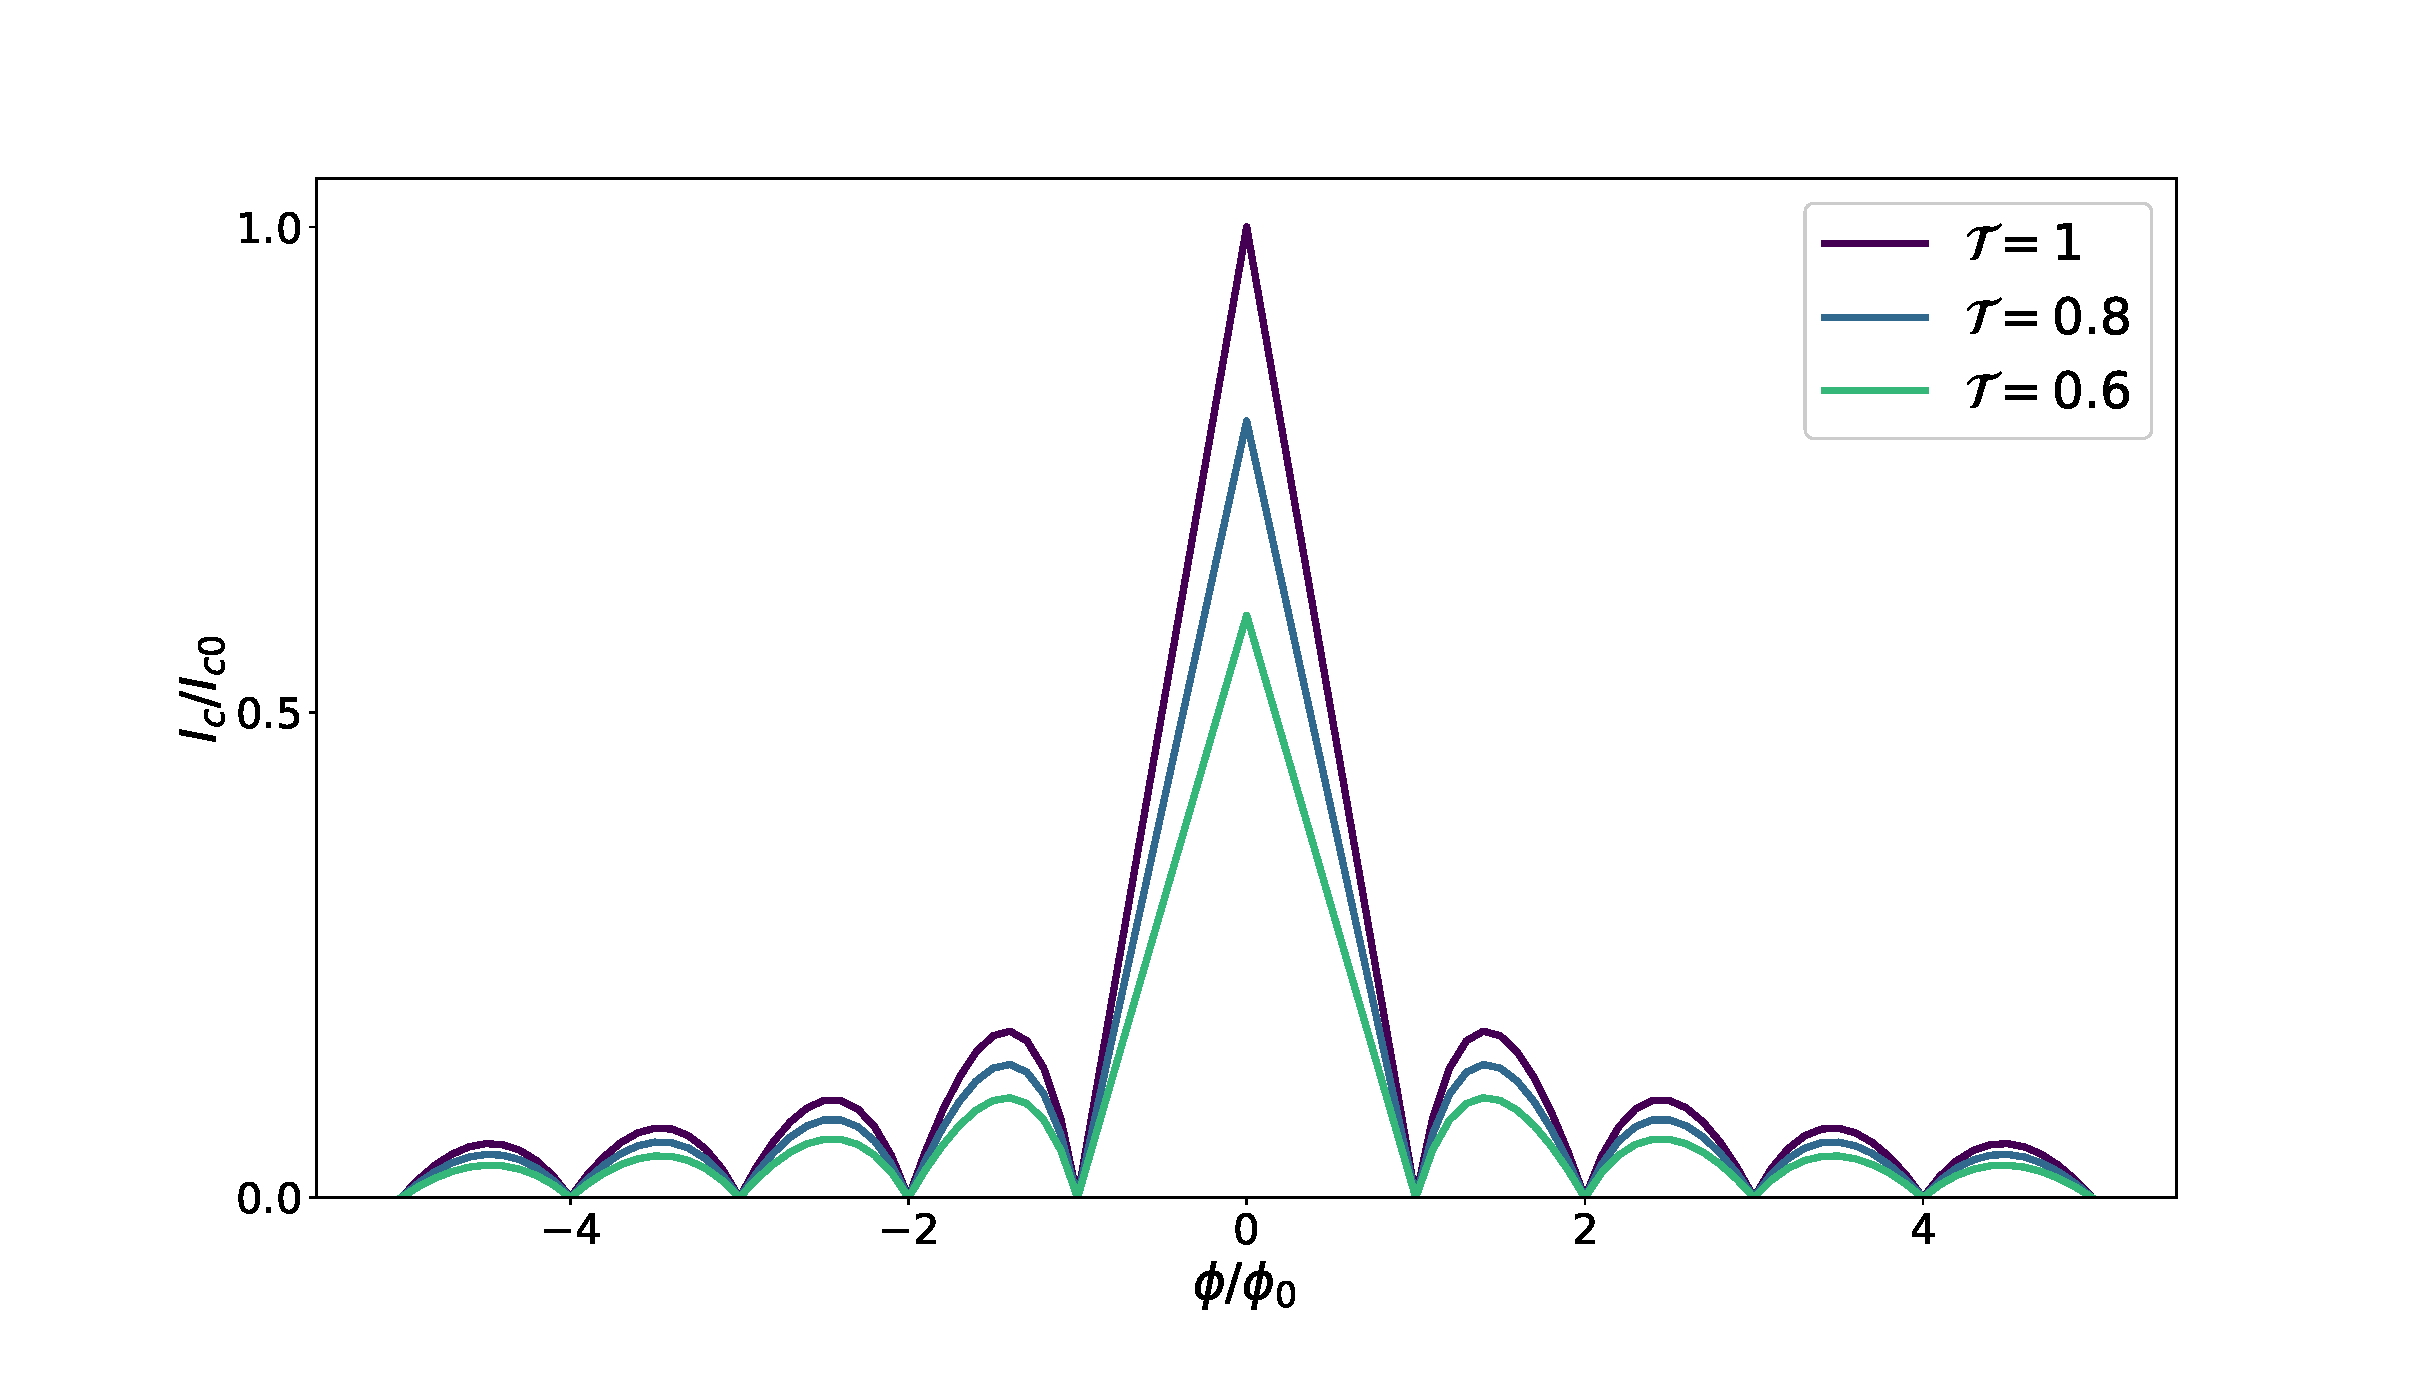
\includegraphics[width=0.9\textwidth]{figure/analyticalmodel/ic_vs_tau}
%\caption{The normed critical current $I_c/I_0$ versus $\phi / \phi_0$ for different transmissions cofficients $\mathcal{T}$. For $\mathcal{T} > 1$, the barrier becomes reflective and the overall current density is low. The sharp peak ar $\phi / \phi_0$ arises from the  }
%\end{minipage}%
%\begin{minipage}{0.5\textwidth}
%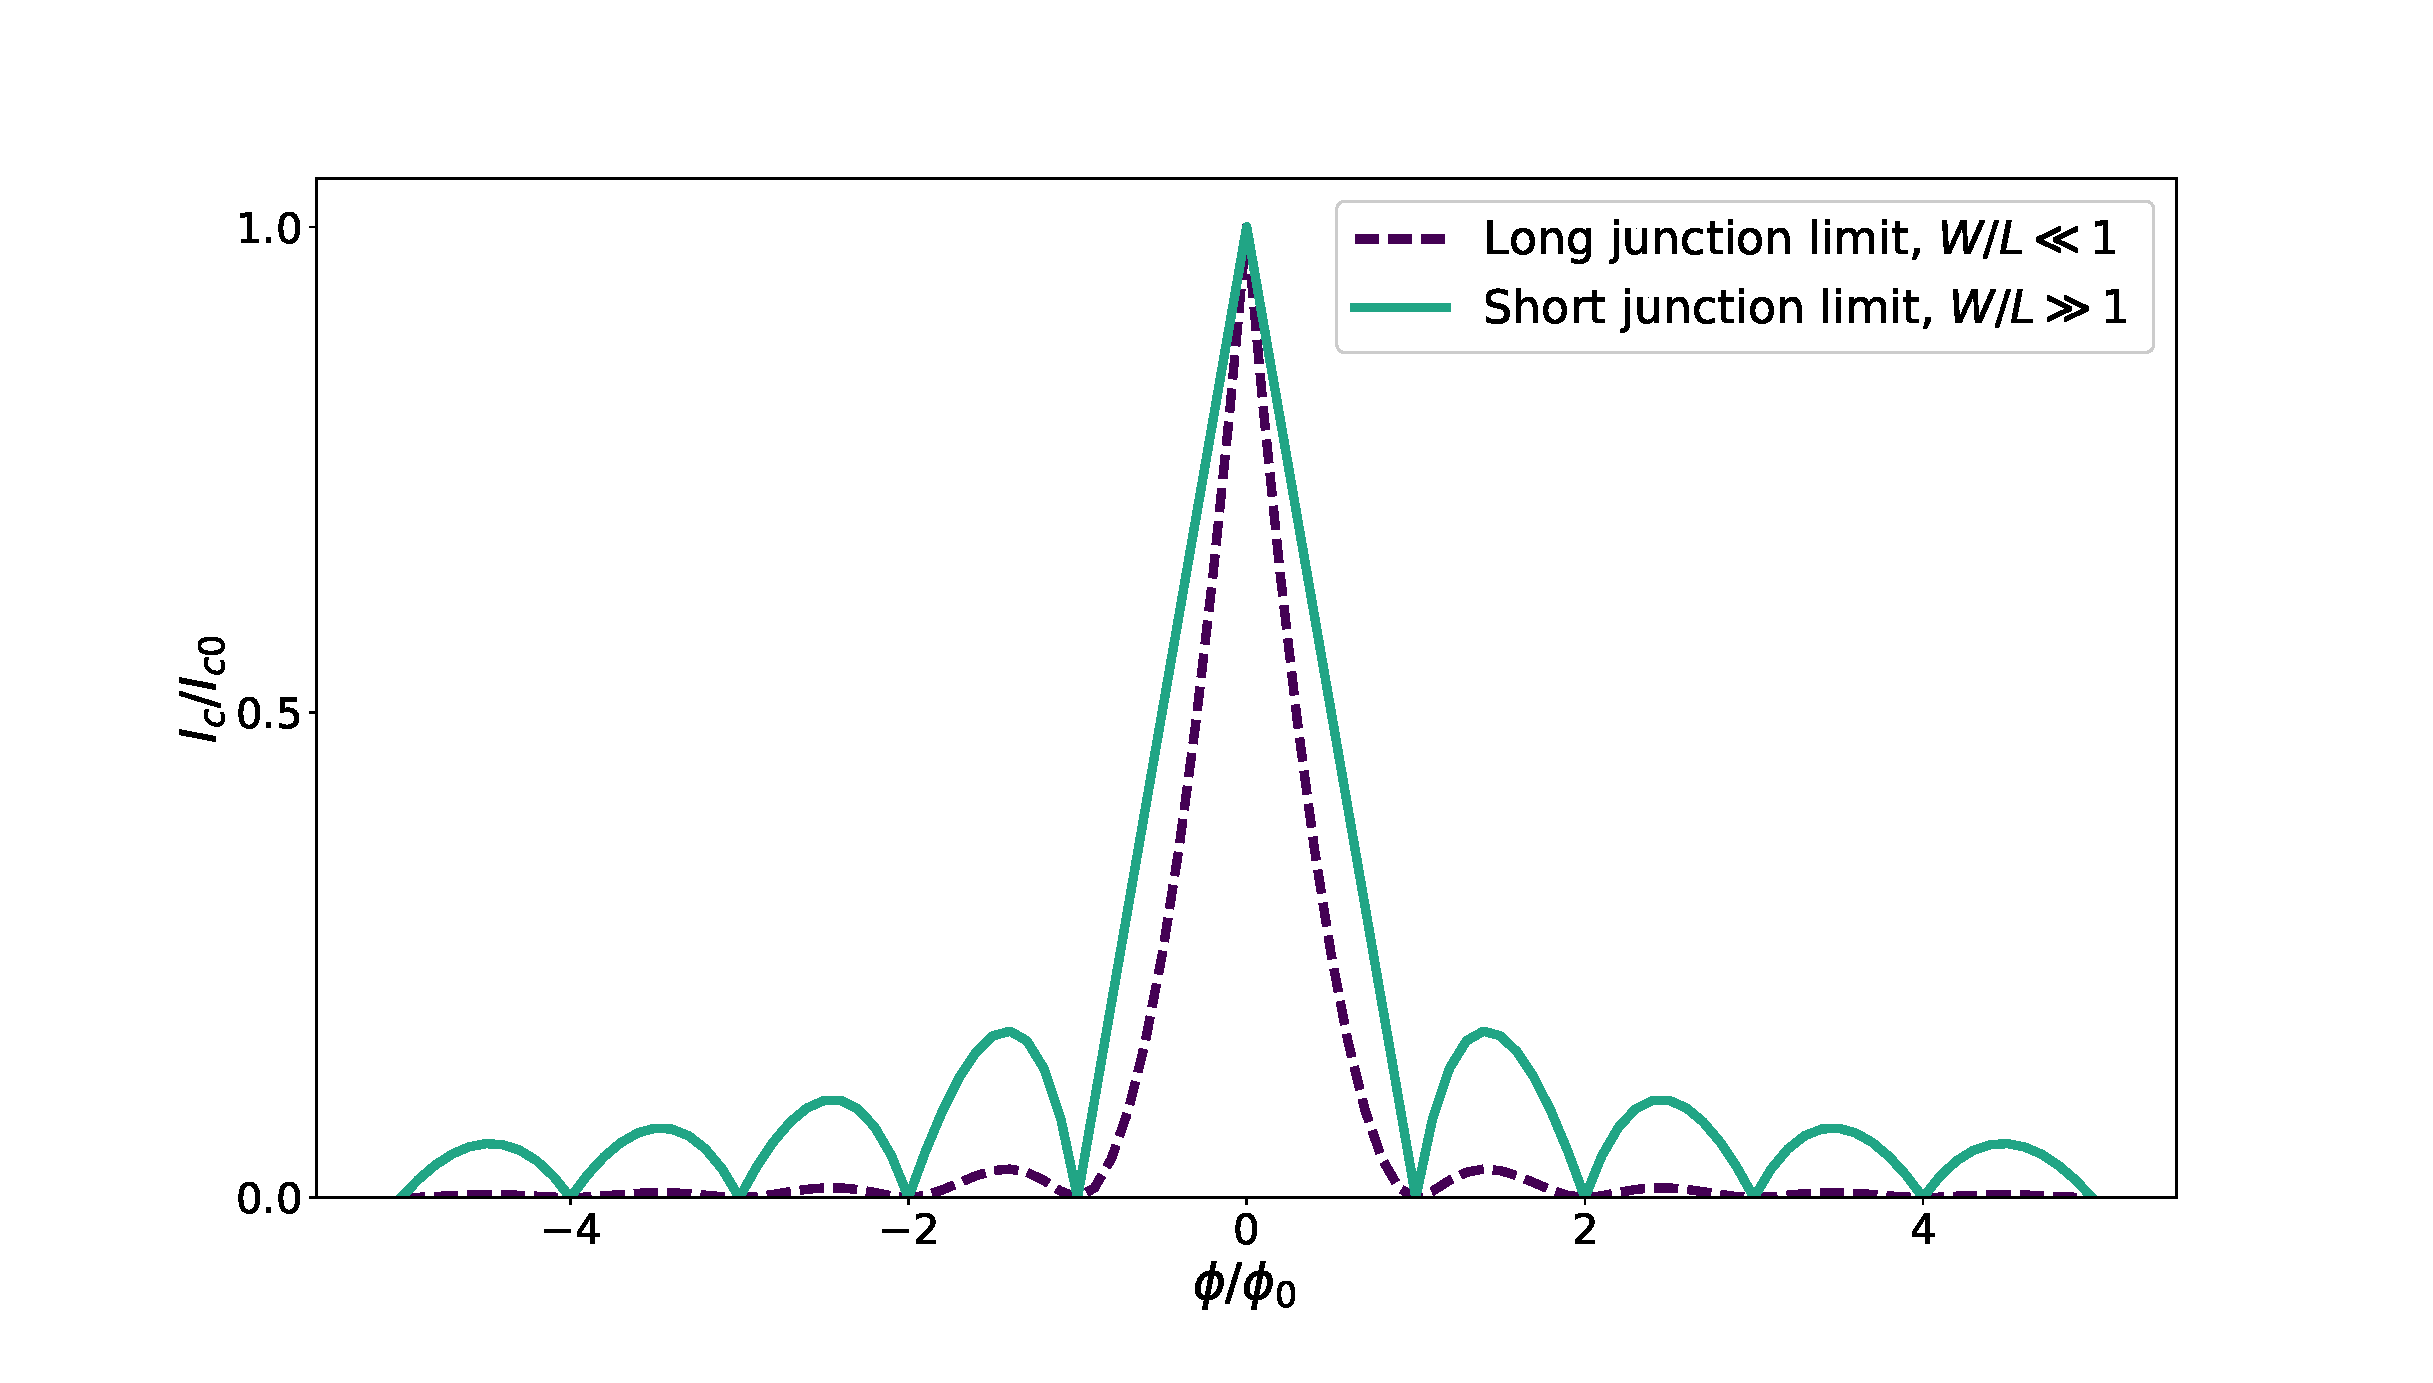
\includegraphics[width=0.9\textwidth]{figure/analyticalmodel/ic-long-vs-short}
%\caption{long vs short}
%\end{minipage}
%\end{figure}

\subsection*{Including Scattering At The Boundaries}
So far, straight trajectories connecting the two superconducting interfaces have been considered. A process that is possible in principal, is a trajectory of an electron that is scattered at a side boundary (at $y = \pm W/2$, see figure \ref{fig:sns_schematic}). It is clear that, especially in the case of a short and wide junction with $W \gg L$, these trajectories do not contribute as much as the straight trajectories. When a trajectory is scattered at, say, a point at the upper edge $(x, y) = (x_s, + W/2)$, the parametrisation for the angle describing the trajectory is
\begin{equation}
\tan \theta = \frac{\bar{y}_2 - y_1}{L} = \frac{W - y_2 - y_1}{L}. \label{eq:angles-scattering}
\end{equation}
In this parametrisation, the coordinate $\bar{y}_2$ is the mirror image of $y_2$. For straight trajectories the vector potential $\mathbf{A}$ does not give an additional contribution, which can be seen in eq. (\ref{eq:magnetic-phase-straight}). The effective phase is in this case determined by eq. (\ref{eq:chi}). When considering the scattering at side boundaries with the parametrization from eq. (\ref{eq:angles-scattering}), the contribution from the magnetic phase is no longer zero,
\begin{eqnarray}
\delta \chi &=& \frac{2 \pi}{\Phi_0} \int_{-L/2}^{x_s} dx A_y(x) \tan \theta  - \frac{2 \pi}{\Phi_0} \int_{x_s}^{+L/2} dx A_y(x) \tan \theta \\
&=& - \frac{2 \pi B }{\Phi_0 } \tan \theta \left( \int_{-L/2}^{x_s} x dx - \int_{x_s}^{+L/2} dx \right) \\
&=& - \frac{2 \pi B}{\Phi_0 } \tan \theta \left( x_s^2 - (L/2)^2 \right) \\
&=& ~ \frac{\pi \phi}{2 W} \frac{(W - 2 y_1) ( W - 2y_2)}{W - y_1 - y_2},
\end{eqnarray}
since the trajectory changes the direction and therefore $d \mathbf{l} \cdot \mathbf{A}$ changes sign. The total effective phase difference is then, using eq. (\ref{eq:chi})
\begin{equation}
\tilde{\chi} (y_1, y_2) = \chi - \frac{\pi \phi}{2 W} \left( 2 (y_1 + y_2) - \frac{(W-2y_1)(W-2y_2)}{W - y_1 - y_2} \right)
\end{equation}
With the contribution from side boundary scattering, the total Josephson current is
\begin{equation}
J \left( \chi, \phi \right) = J^{(0)} \left( \chi, \phi \right)  + 2 J^{(1)} \left( \chi, \phi \right).\label{eq:total-current}
\end{equation}
$J^{(0)}$ denotes the part coming from straight trajectories. Since there are two side boundaries, the part describing the scattering, $J^{(1)}$, has an additional factor 2 and reads
\begin{equation}
J^{(1)} = \frac{2 e v_F}{\pi \lambda_F L^2} \int \int_{-W/2}^{W/2} \frac{d y_1 d y_2}{ \left[ 1 + \left(\frac{y_1 - y_2}{L}\right)^2\right]^{2}} \mathcal{J} \left( \chi - \frac{\pi \phi}{2 W} \left( 2 (y_1 + y_2) - \frac{(W-2y_1)(W-2y_2)}{W - y_1 - y_2} \right)\right) \label{eq:josephson-edge}
\end{equation}
This contribution has not been noted in \cite{Meier2016}. In the case of short and wide junctions, it is sufficient to consider only $J^{(0)}$. For the cases, when $W / L \simeq 1$, it is necessary to sum over all possible edge channels.
\begin{figure}
\centering
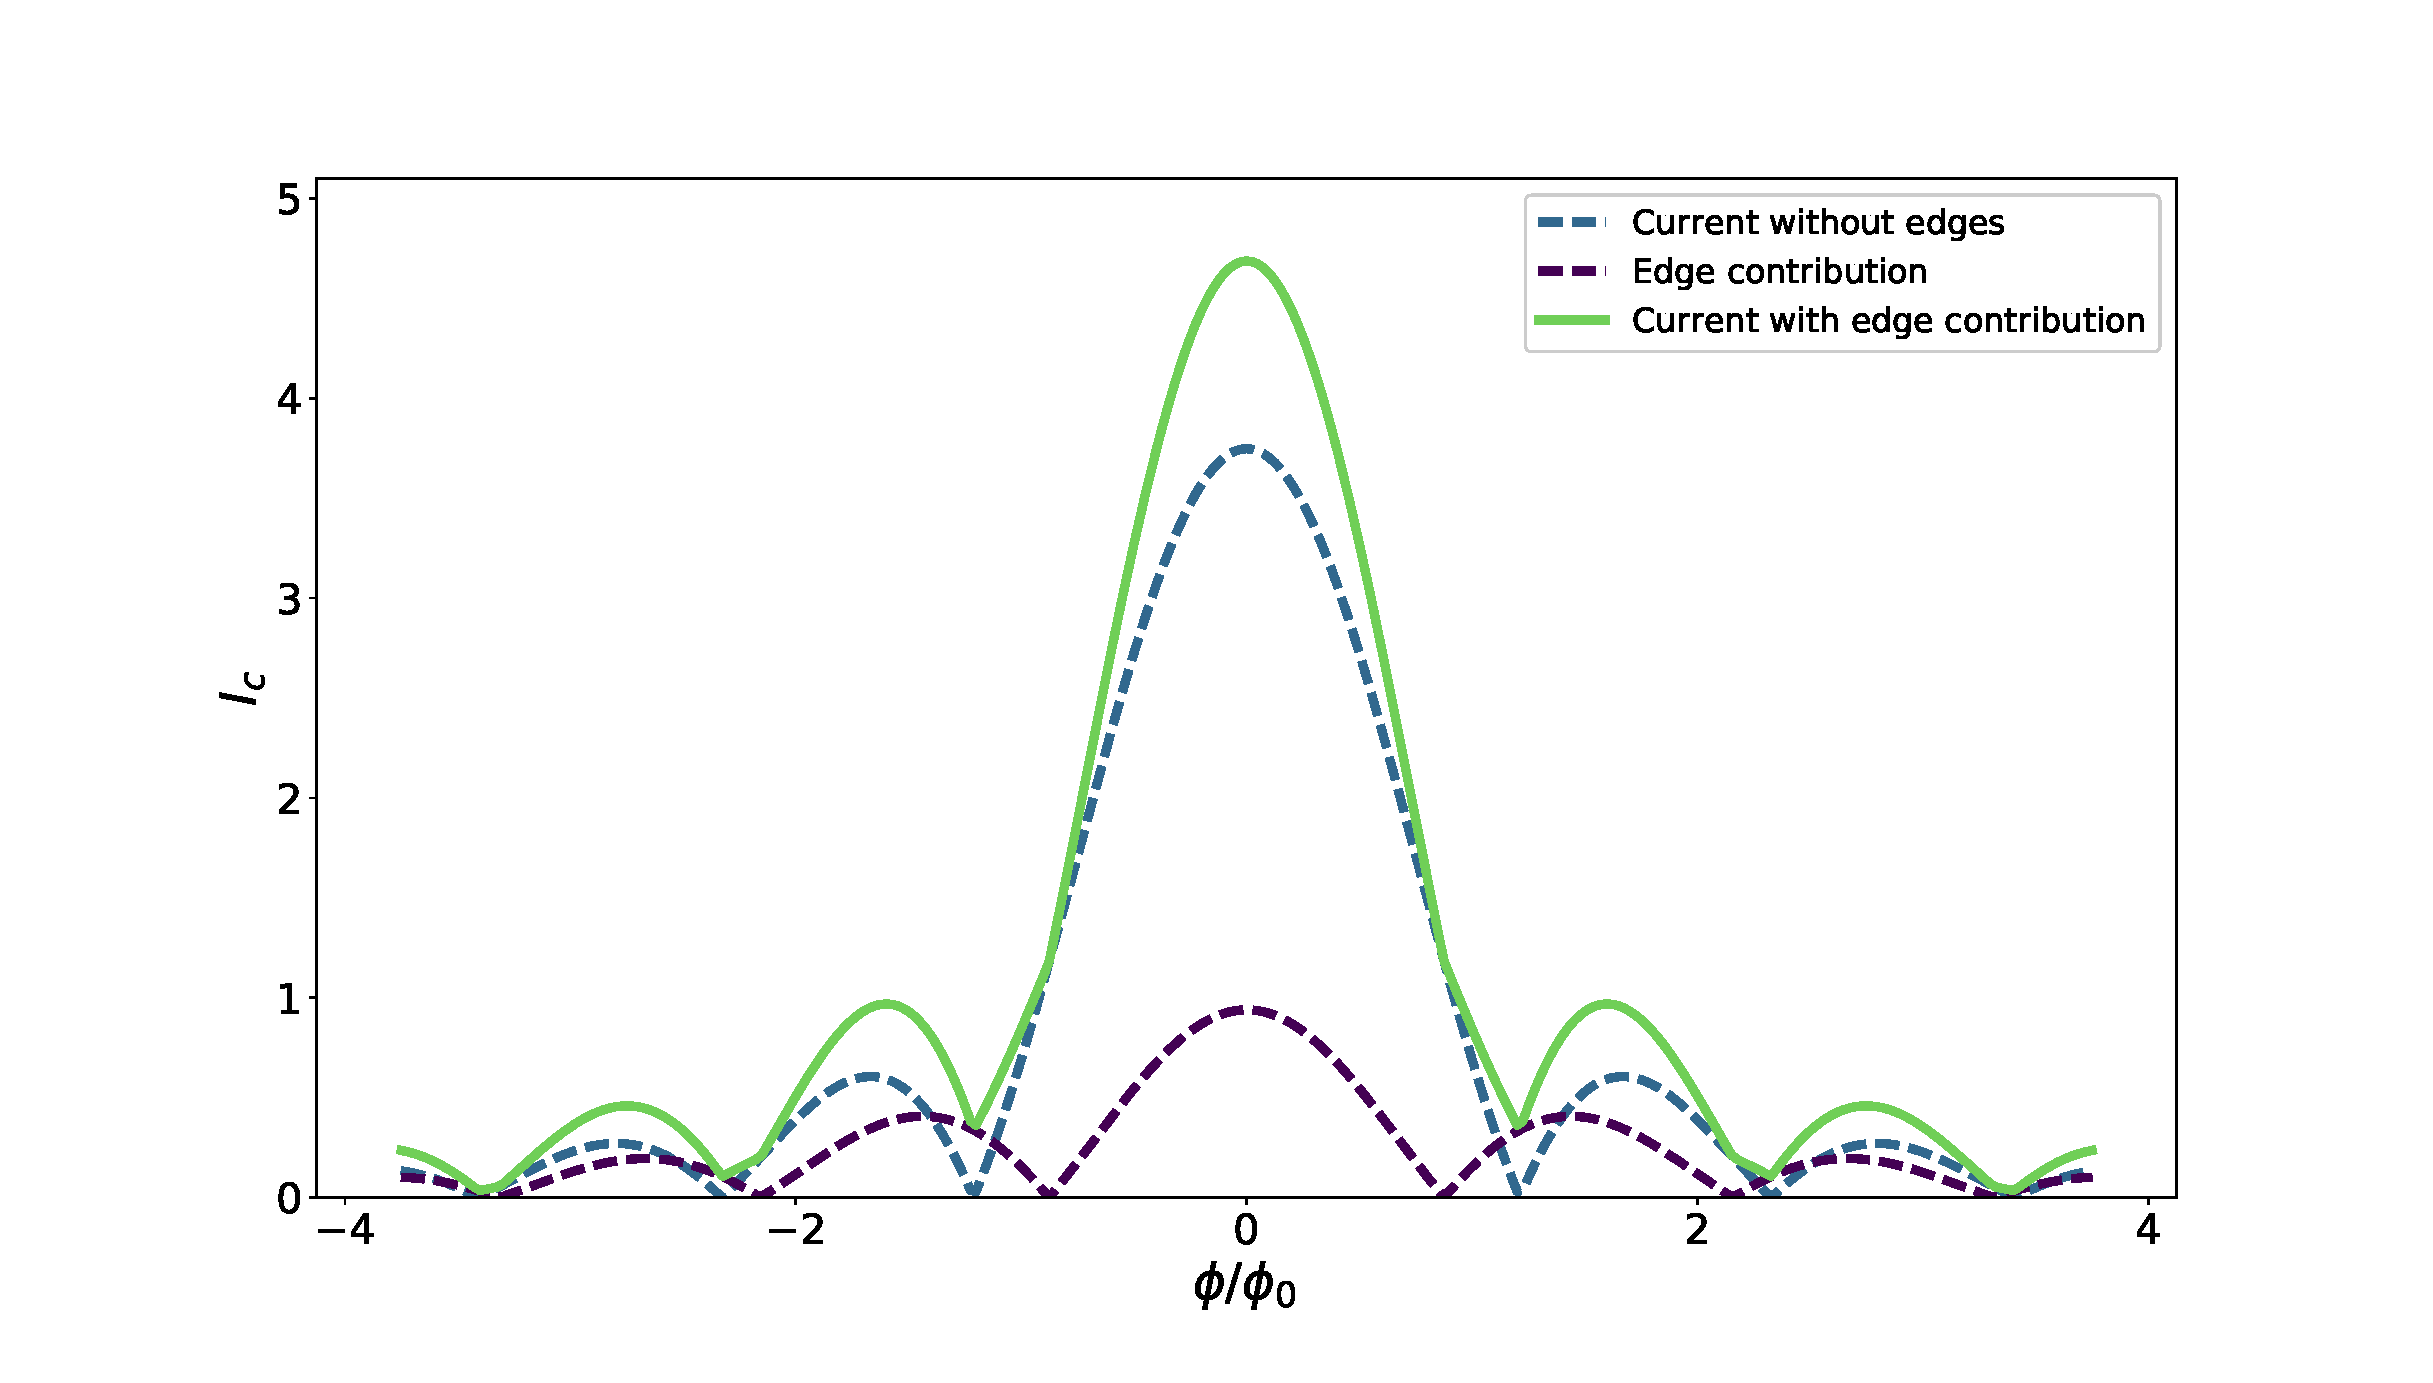
\includegraphics[width=\textwidth]{figure/analyticalmodel/plane-setup-edge-contribution}
\caption{Comparison of contribution  to current with and without boundary scattering at $\mathcal{T} =1$. The total current is a sum of the contribution without boundary scattering, $I_c^{(0)}$, and two times the current from the boundaries, $I_c^{(1)}$. The boundary scattering can be seen in the Fraunhofer pattern of the total current in the lifting of the lobes}\label{fig:plane-edge-contribution}
\end{figure}
Figure \ref{fig:plane-edge-contribution} shows the result of equations (\ref{eq:josephson-edge}) and (\ref{eq:josephson_current}). The overall contribution from the side scattering is lower than the contribution of only straight trajectories. In the total current, eq. (\ref{eq:total-current}), the edge scattering manifests by lifting the minimas from zero (see green curve in figure \ref{fig:plane-edge-contribution}). This is in agreement with the results from \cite{Meier2016}

\section{Calculation Of The QPC Critical Current}
\begin{figure}
\centering
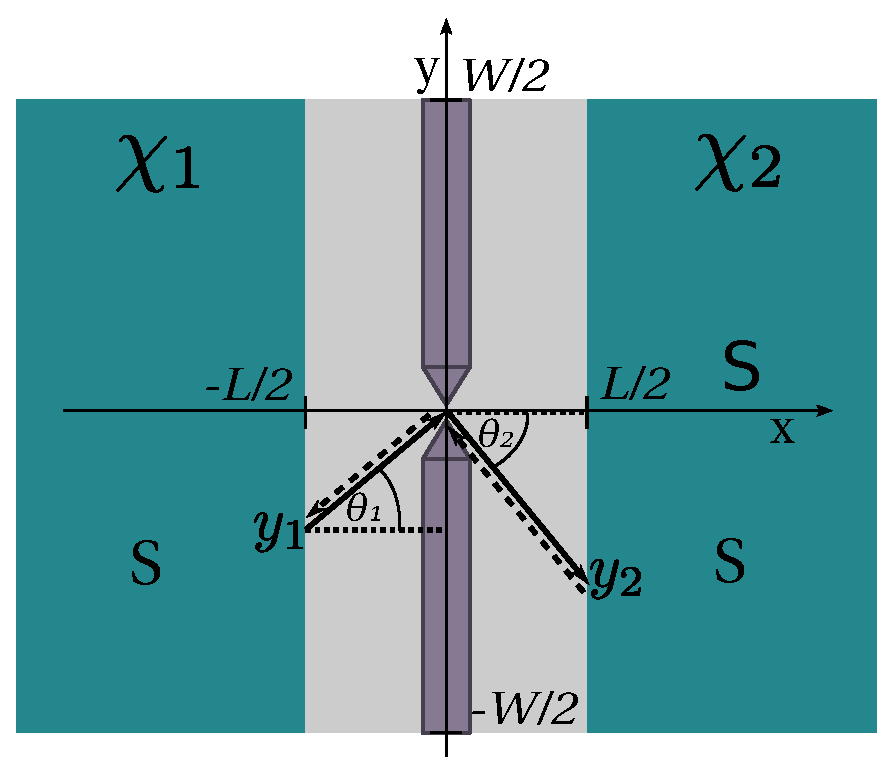
\includegraphics[width=0.6\textwidth]{figure/analyticalmodel/qpc_sns_junction_csch}
\caption{SNS junction with a QPC gate on top. The split is located at $(x, y) = (0, 0)$, and the width of the barrier is assumed to be negligible. Each contributing trajectory has to pass though the origin. The angles $\theta_1$ and $\theta_2$ parametrize this trajectory.}
\label{fig:qpc_sns_schematic}
\end{figure}
%\textbf{TODO: what happens when a constriction is on top of normal layer, fermi levels etc}
The quasi classical formalism can even be employed to modified SNS junctions. One can build gates on top of the normal region of the junction in a way that the current cannot pass through the gated regions (see chapter \ref{ch:experiment}). In the quasi classical picture, this means that the possibilities for trajectories connecting two points at the superconducting interfaces are limited through the geometry of the constriction.\\
Figure \ref{fig:qpc_sns_schematic} shows a sketch of the quantum point contact set-up which will be analysed with the quasi classical formalism. The normal region of the SNS junction is covered by a gate with a small split in the middle. The split is located at $(x, y) = (0, 0)$ so that the sample is symmetric around the origin. The width of the split is in the order of $\lambda_F$  and can thereby be viewed as an isotropic scattering point with transmission coefficient $\mathcal{T}_0$. Trajectories connecting the two superconducting interfaces have to pass through the QPC. For simplicity, the geometrical width of the barrier is neglected, only straight trajectories are considered, and scattering at side edges is neglected. This modified set-up leads to a different parametrization of the trajectories and therefore to a different magnetic phase than in eq. (\ref{eq:chi}).\\
With the QPC set-up, all possible trajectories are parametrized by two angles $\theta_1$ and $\theta_2$. $\theta_1$ describes the trajectory before passing through the QPC in the region $ -L/2 < x < 0$, and  $\theta_2$ after passing through the QPC. The parametrization of the trajectories reads
\begin{equation}
\tan \theta_1 = - \frac{2 y_1}{L}, \quad \tan \theta_2 = \frac{2 y_2}{L}
\label{eq:QPCparametrization}
\end{equation}
With the gauge from eq. (\ref{eq:Ay}), the magnetic phase acquired within the sample reads
\begin{eqnarray}
\frac{2\pi}{\Phi_0} \int d\mathbf{l} \cdot \mathbf{A}  &=&
-\frac{\pi B}{\Phi_0}\left(\frac{L}{2}\right)^2
\left(-\tan\theta_1 + \tan\theta_2\right) =
-\frac{\pi \phi (y_1+y_2)}{2 W}.
\label{eq:phaseQPC}
\end{eqnarray}
The total phase difference is the difference of the contribution coming from the magnetic field, eq. (\ref{eq:phaseQPC}) and the superconducting phase difference eq.~(\ref{eq:chi}). The effective phase for the QPC set-up is found to be
\begin{equation}
\tilde{\chi}(y_1,y_2)=\chi-\frac{ \pi \phi }{2W}(y_1+y_2).
\label{eq:chiQPC}
\end{equation}
%The contribution in eq. (\ref{eq:chiQPC}) is half of the effective phase without any constriction, as written in eq. (\ref{eq:chi}). This is reasonable and can be illustrated by looking at the area contributing to the phase. Only half of the normal region is covered by all possible trajectories in the QPC case, whereas in the case without any constriction, the whole normal region contributes.\\
%\textbf{TODO: stimmt das da oben? warum?}\\
One consequence of the additional gate on top of the normal region is the change in the effective phase, resulting in a modified current phase relation $\mathcal{J}(\tilde{\chi}(y_1, y_2))$. Another consequence is a modified expression for the critical current. In the set-up without gates, straight trajectories with a fixed angle $\theta$ were considered and summed up to a total contribution. The difference in the QPC set-up is the split in the gate, which is modelled as an isotropic scattering point. The trajectories being summed up in this set-up can be thought to consist of two parts. The first part connects $y_1$ with the split at $(x, y) = (0, 0)$ and is determined by the direction of the trajectory. This explains the Fermi velocity in this part(?). The second part of the current trajectory starts from the origin and connects it with a point at the right interface $y_2$. Summing up, the  critical current in the QPC set-up is
\begin{equation}
I_c^{\text{QPC}}(\phi) \propto \text{max}_{\chi} \int d \theta_1 v_F \cos^2 \theta_1 \int d \theta_f \cos \theta_f \mathcal{J}\left( \tilde{\chi} (\theta_1, \theta_2) \right)
\end{equation}
%The normalized critical current reads
%\begin{eqnarray}
%\frac{I_c(\phi)}{I_c(0)} &=& \frac{ \text{max}_{\chi} \int d \theta_i \cos^2 \theta_i\int d \theta_f \cos \theta_f \mathcal{J}(\tilde{\chi}(\theta_i, \theta_f)) }{ \text{max}_{\chi} \int d \theta_i \cos^2 \theta_i\int d \theta_f \cos \theta_f \mathcal{J}(\chi) }
%\end{eqnarray}
The QPC is modelled as an isotropic scatterer with transmission probability $\mathcal{T}$. If the transmission is small, $\mathcal{T} << 1$, eq.~(\ref{eq:josephson-low-t}) can be used for $\mathcal{J}$.
%TODO \textbf{TODO: add why from $\sin \tilde{\chi}$ only cosine survives!}
The angles $\theta_{1, 2}$ can be rewritten in terms of $y_{1, 2}$ by using the parametrization from eq.~(\ref{eq:QPCparametrization}), allowing the normalized critical current to be expressed as
\begin{eqnarray}
\frac{I_c(\phi)}{I_c(0)} &=& \frac{\mathcal{I}_2(\phi)\mathcal{I}_{3/2}(\phi)}{\mathcal{I}_2(0)\mathcal{I}_{3/2}(0)}\label{eq:qpc-integral},
\end{eqnarray}
where the integrals $\mathcal{I}$ are defined as
\begin{equation}
\mathcal{I}_k(\phi) = \frac{2}{L}\int_{-W/2}^{+W/2}dy \frac{\cos\left(\frac{\pi\phi y}{2W}\right)}{\left[1 + \left(\frac{2y}{L}\right)^2 \right]^k}
\label{integral-qpc}
\end{equation}

Evaluating the integral in eq. (\ref{eq:qpc-integral}) numerically gives a bell-shaped form that is very well described with a Gaussian function $\exp ( -a (x-\mu)^2 / (2 \sigma)^2 )$. Figure \ref{fig:ic-qpc-gauss} shows a plot of the resulting current from the integration as well as a plot of the fitted function. 
\begin{figure}
\centering
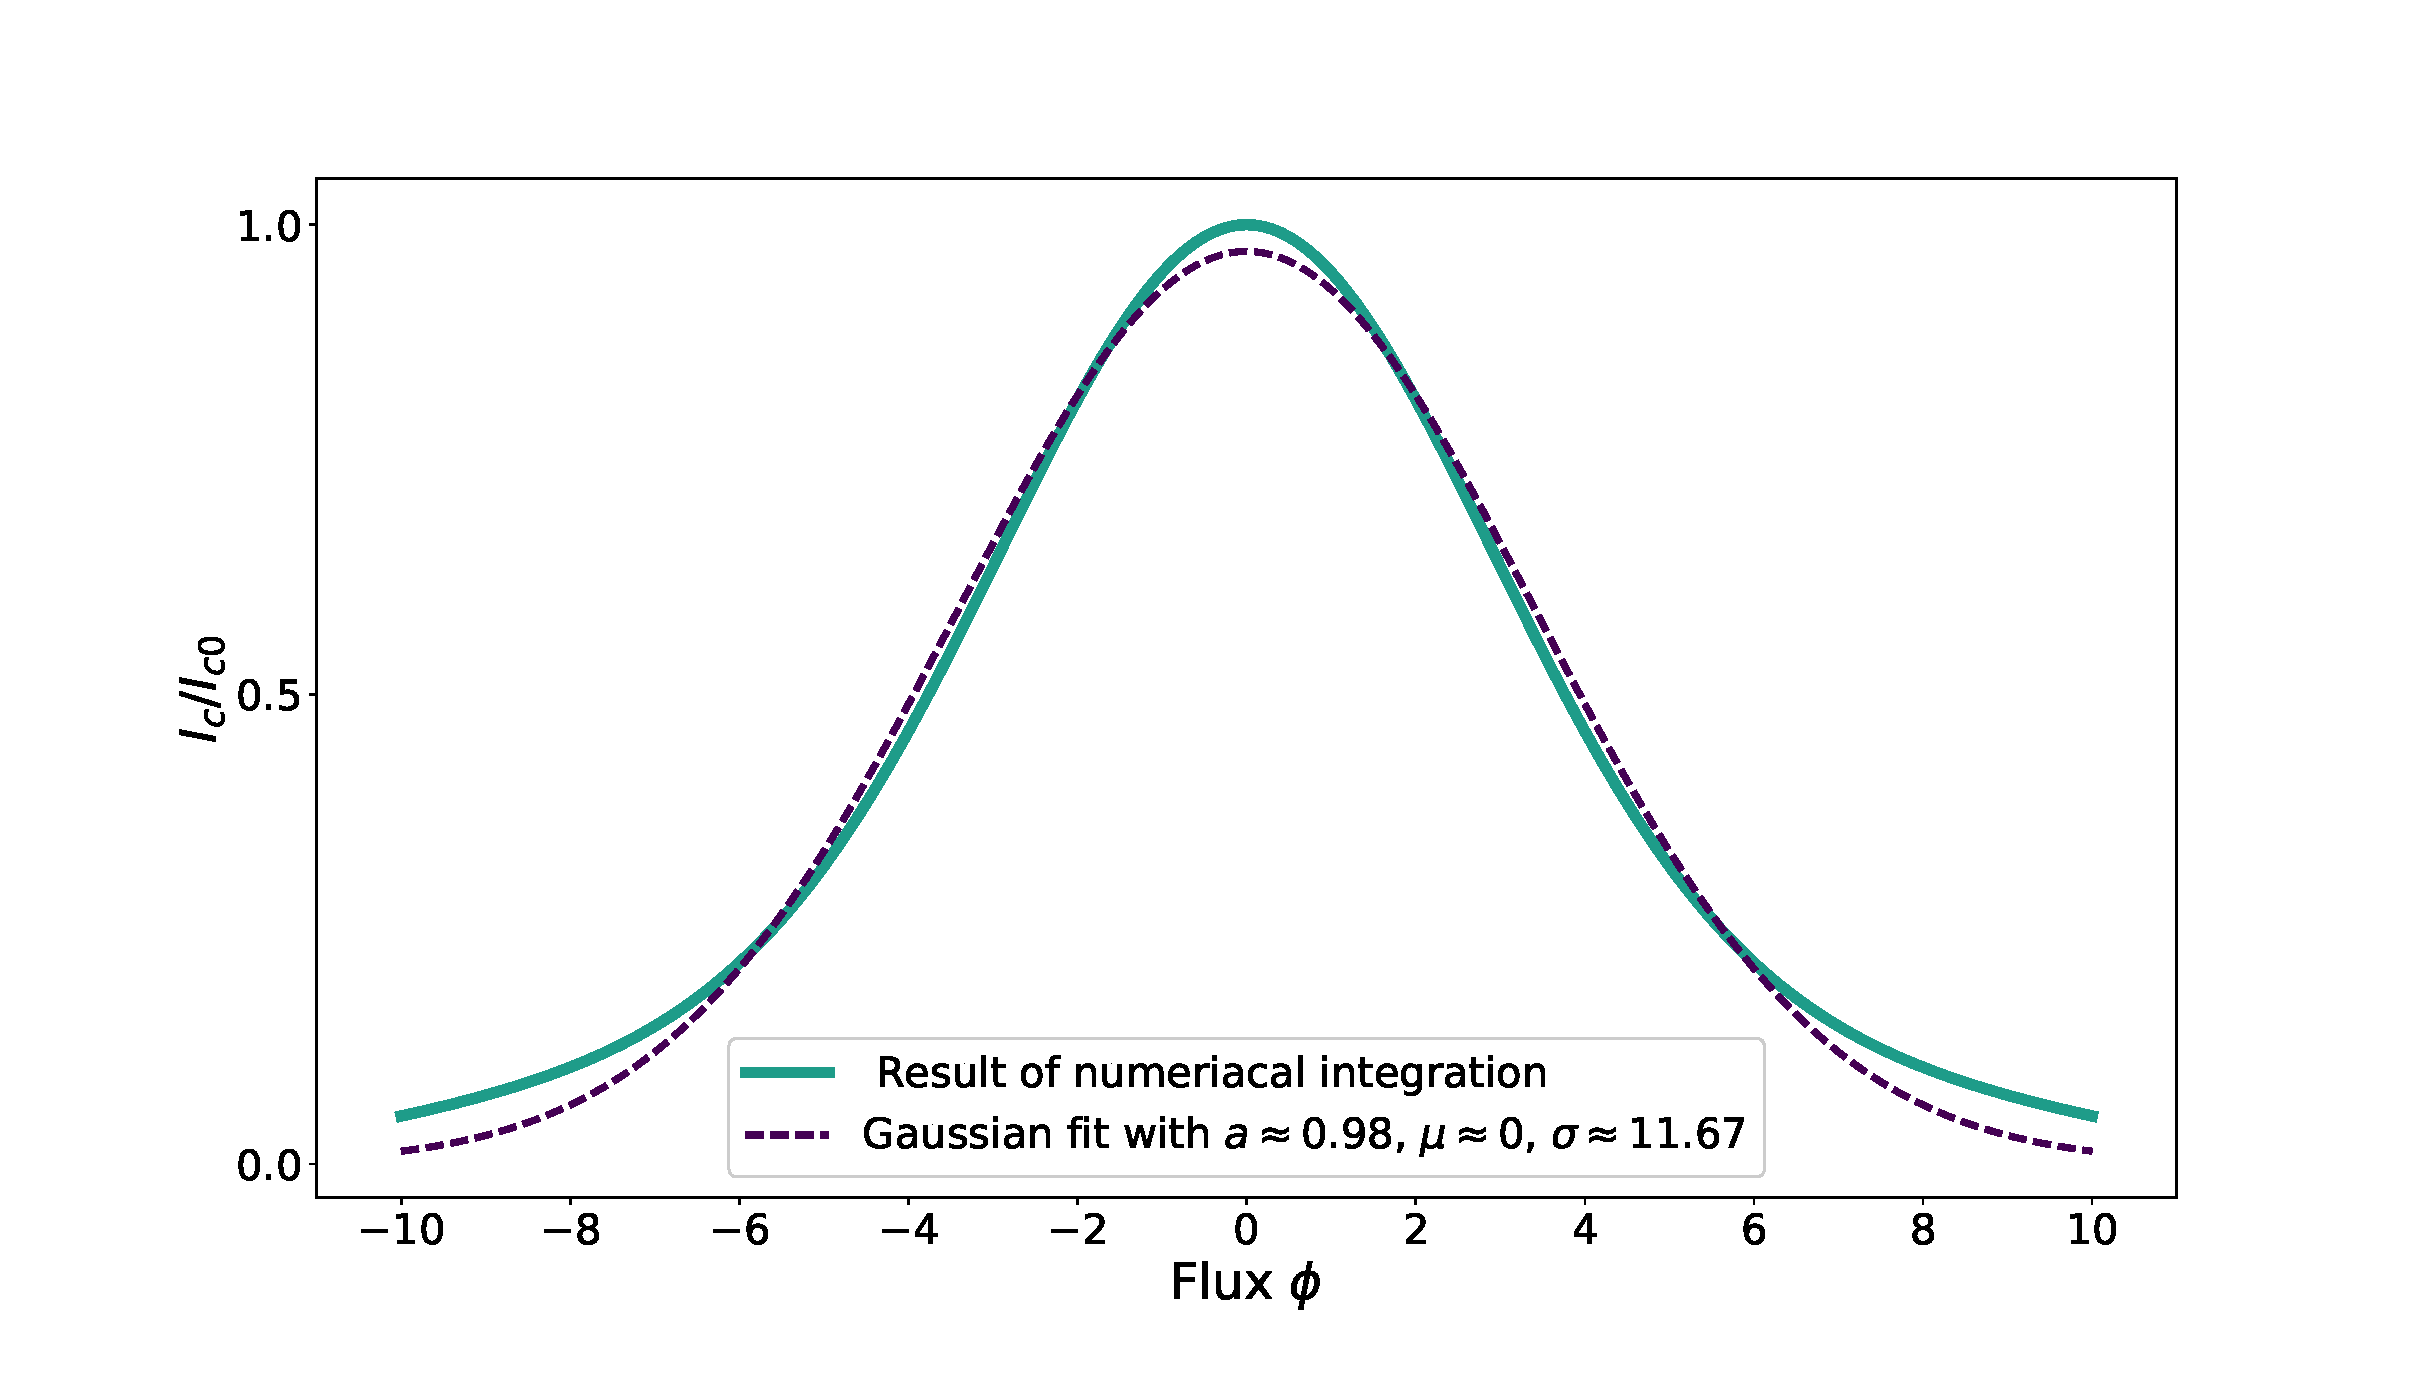
\includegraphics[width=0.6\textwidth]{figure/analyticalmodel/qpc-numerical-integration-fit}
\caption{Plot of the numerical integration for the QPC current from eq. (\ref{eq:qpc-integral}) and the result of the fitting to a Gaussian curve.} \label{fig:ic-qpc-gauss}
\end{figure}
\subsubsection*{Evaluation In Limits}
The current can be evaluated in the limit of small flux $\phi \rightarrow 0$, and in limit of high fields $\phi \rightarrow \infty$. 
At $\phi=0$ the cosine term becomes one leading to the simple expression
\begin{eqnarray}
\mathcal{I}_2(0)\mathcal{I}_{3/2}(0) &=&
\frac{2 W^2 L}{\left( L^2 + W^2 \right)^{3/2}} + \frac{2W}{\sqrt{L^2 + W^2}} \arctan \frac{W}{L}  \\
&\equiv & \frac{2 x^2}{\left( 1 + x^2 \right)^{3/2}} + \frac{2 x}{\sqrt{1 + x^2} } \arctan x,
\label{Ic-0}
\end{eqnarray}
where $x \equiv W/L$.
The parabolic asymptotics of the critical current at small $\phi$ is found by expanding the cosine factors in the numerator:
\begin{eqnarray}
\frac{I_c(\phi)}{I_{c0}}&\simeq& 1 - \frac{\pi ^2 \phi^2 }{32} f_0(W/L) \\
f_0(x) &=& \frac{\sqrt{x^2+1} \log \left(\sqrt{x^2+1}+x\right)}{x^3} - \frac{2}{x (x+(x^2+1) \arctan x)} 
\end{eqnarray}
In the opposite limit of high fields, $\phi\to \infty$, the integration in eq.~(\ref{integral-qpc}) is extended over $y_1$ and $y_2$ to $\pm \infty$ and obtain
\begin{eqnarray}
\frac{I_c(\phi)}{I_{c0}} &=& \frac{\pi^{3/2}}{8 x} \frac{(1 + x^2)^{3/2}}{x + (1+x^2) \arctan x} \left( \frac{\pi \phi}{2 x} \right)^{3/2} \exp \left( - \frac{\pi \phi}{2 x} \right)
\label{eq:large-phi}
\end{eqnarray}


\section{QPC Edge Current}
The role of edge current is of importance when studying SNS junctions. As has been explained in chapter \ref{ch:experiment}, when a large band gap is opened in BLG, an insulating state is expected, especially at very low temperatures. The non-occurrence of this insulating state has been attributed to the existence of edge currents in the sample. It makes sense to address the problem also for the QPC in within the quasi-classical framework. To this end, two scattering points at the edges $(x, y) = (0, \pm W/2)$ are introduced. These scattering points are modelled in the exact same way as the QPC (they are assumed to be isotropic scatterers) and only differ by means of transmission coefficient. The edge channel transmission coefficient is denoted with $\mathcal{T}_e$ and the QPC transmission coefficient with $\mathcal{T}_q$. 

\begin{figure}
\centering
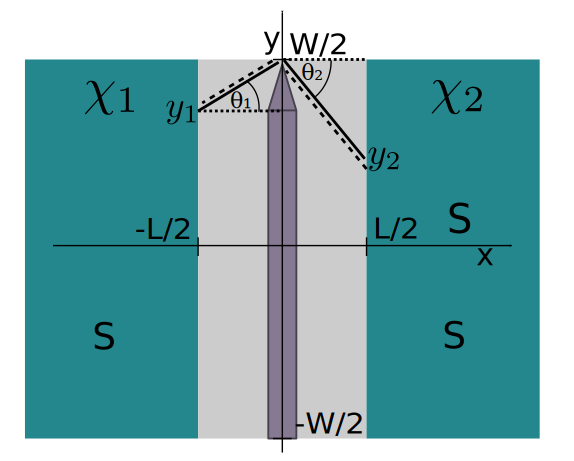
\includegraphics[width=0.6\textwidth]{figure/analyticalmodel/qpc_edges_angles_csch}
\caption{A SNS junction with split at upper edge, $(x, y) = (0, + W/2)$. Similar to the QPC set-up, this constriction is formed so that each trajectory has to pass through in order to contribute to the current.}\label{fig:qpc-edge-parametrization}
\end{figure}
The parametrization of an edge trajectory, illustrated in figure \ref{fig:qpc-edge-parametrization}, reads
\begin{eqnarray}
\tan \theta_1 = ~\frac{ W - y_1}{L/2}, \quad \tan \theta_2 = -\frac{W - y_2}{L/2} \label{eq:angles-edge}.
\end{eqnarray}
Similar to the QPC contribution, the magnetic phase gain along the trajectory is calculated. For the upper edge, the result is
\begin{eqnarray}
\frac{2 \pi}{\phi_0} \int d \mathbf{l} \cdot \mathbf{A} &=& \frac{2 \pi}{\phi_0} \left( \int A_y(x) |d\mathbf{l}| |\mathbf{e_y}| \sin \theta_1 + \int A_y(x) |d\mathbf{l}| |\mathbf{e_y}| \sin \theta_2  \right)\\
%&=& \frac{2 \pi B}{\phi_0} \left( \int_{-L/2}^{0} \frac{x dx}{\cos \theta_1} \sin \theta_1  + \int_{0}^{L/2} \frac{x dx}{\cos \theta_2} \sin \theta_2 \right) \\
&=&  - \frac{2 \pi B}{\phi_0} \left( \int_{-L/2}^{0} x dx \tan \theta_1 + \int_{0}^{L/2} x dx \tan \theta_2 \right) \\
&=&  - \frac{\pi B}{\phi_0} \frac{L}{2} \left( - \tan \theta_1 + \tan \theta_2 \right) \\
&=& - \frac{\pi B}{\phi_0} \frac{L}{2} \left( -2W + (y_1 + y_2) \right)\\
&=& \pi \Phi -\frac{\pi \Phi }{2 W} (y_1 + y_2),
\end{eqnarray}
where
\begin{equation}
\Phi = \frac{\phi}{\phi_0}, \quad \phi = B W L
\end{equation}
has been used. Together with the contribution from the set-up without any constriction from eq.~(\ref{eq:chi}), the total phase for the edge transmission is added up to
\begin{equation}
\tilde{\chi}(y_1, y_2) = \chi - \frac{3 \pi \Phi}{2\phi_0} (y_1 + y_2) + \pi \Phi \label{eq:chi-edge}.
\end{equation}
This is the effective phase $\tilde{\chi}(y_1, y_2)$ for the upper edge leading to a critical current $I_c^{e, u}$. Analogously, the phase for the lower edge can be constructed with a simple sign change in the parametrization in eq. (\ref{eq:angles-edge}):
\begin{equation}
\tilde{\chi}(y_1, y_2) = \chi + \frac{3 \pi \Phi}{2\phi_0} (y_1 + y_2) - \pi \Phi,
\end{equation}
which is the effective phase for the lower edge current, $I_c^{e, l}$.
The Josephson relation for the edge contribution has the modified phase from eq. (\ref{eq:chi-edge}). 
The result for the QPC in the limit in high fields, eq. (\ref{eq:large-phi}), has a transmission coefficient $\mathcal{T} = 1$. For easier comparison with the edge channel contribution, this is rewritten into the following form
\begin{equation}
I_c^{\text{QPC}} = \mathcal{T}_q F(W/L),
\end{equation}
where the function $F(W/L)$ represents the result from eq. (\ref{eq:large-phi}). The integrals for the upper edge can be written in a similar way:
\begin{eqnarray}
I_c^{e, u} &=& \mathcal{T}_e \text{max}_{\chi} \{ \sin \left( \chi_0 - \pi \Phi \right) \int_0^\infty d \tilde{y}_1 \int_0^\infty d \tilde{y}_2 \frac{\cos \left( \frac{3 \pi \Phi \tilde{y}_1}{2 W} \right) }{\left( 1 + \left( \frac{2 \tilde{y}_1}{L}\right)^2 \right)^2} \frac{\cos \left( \frac{3 \pi \Phi \tilde{y}_2}{2 W} \right)}{\left( 1 + \left( \frac{2 \tilde{y}_1}{L}\right)^2 \right)^{3/2}} \}\\
&=& \mathcal{T}_e \text{max}_{\chi} \left\{ \sin \left( \chi - \pi \Phi \right) \right\} \frac{F(W/L)}{4}, 
\end{eqnarray}
where
\begin{equation}
\tilde{y}_{1/2} = W/2 - y_{1/2}.
\end{equation}
The total critical though the junction is proportional to the sum of the individual contributions of the QPC, the upper edge, and the lower edge: $I_c^\text{total} = I_c^\text{QPC} + I_c^{e,u} + I_c^{e,l}$. The normalized total current then is
\begin{eqnarray}
\frac{I_c^\text{total}\left( \phi \right)}{I^\text{total}_{c0}} &=& \text{max}_\chi \left\{ \mathcal{T}_q \sin \chi + \frac{\mathcal{T}_e}{4} \sin \left( \chi - \pi \phi \right) + \frac{\mathcal{T}_e}{4} \sin \left( \chi + \pi \phi \right) \right\} / \left( \mathcal{T}_q + \mathcal{T}_e/2 \right)\\
&=& \frac{| \mathcal{T}_q / \mathcal{T}_e + \cos \left( \pi \phi \right)/2 |}{\mathcal{T}_q / \mathcal{T}_e + 1/2}\label{eq:ratio-transmissions} \\
&\equiv & \mathcal{C}
\end{eqnarray}

\begin{figure}
\centering
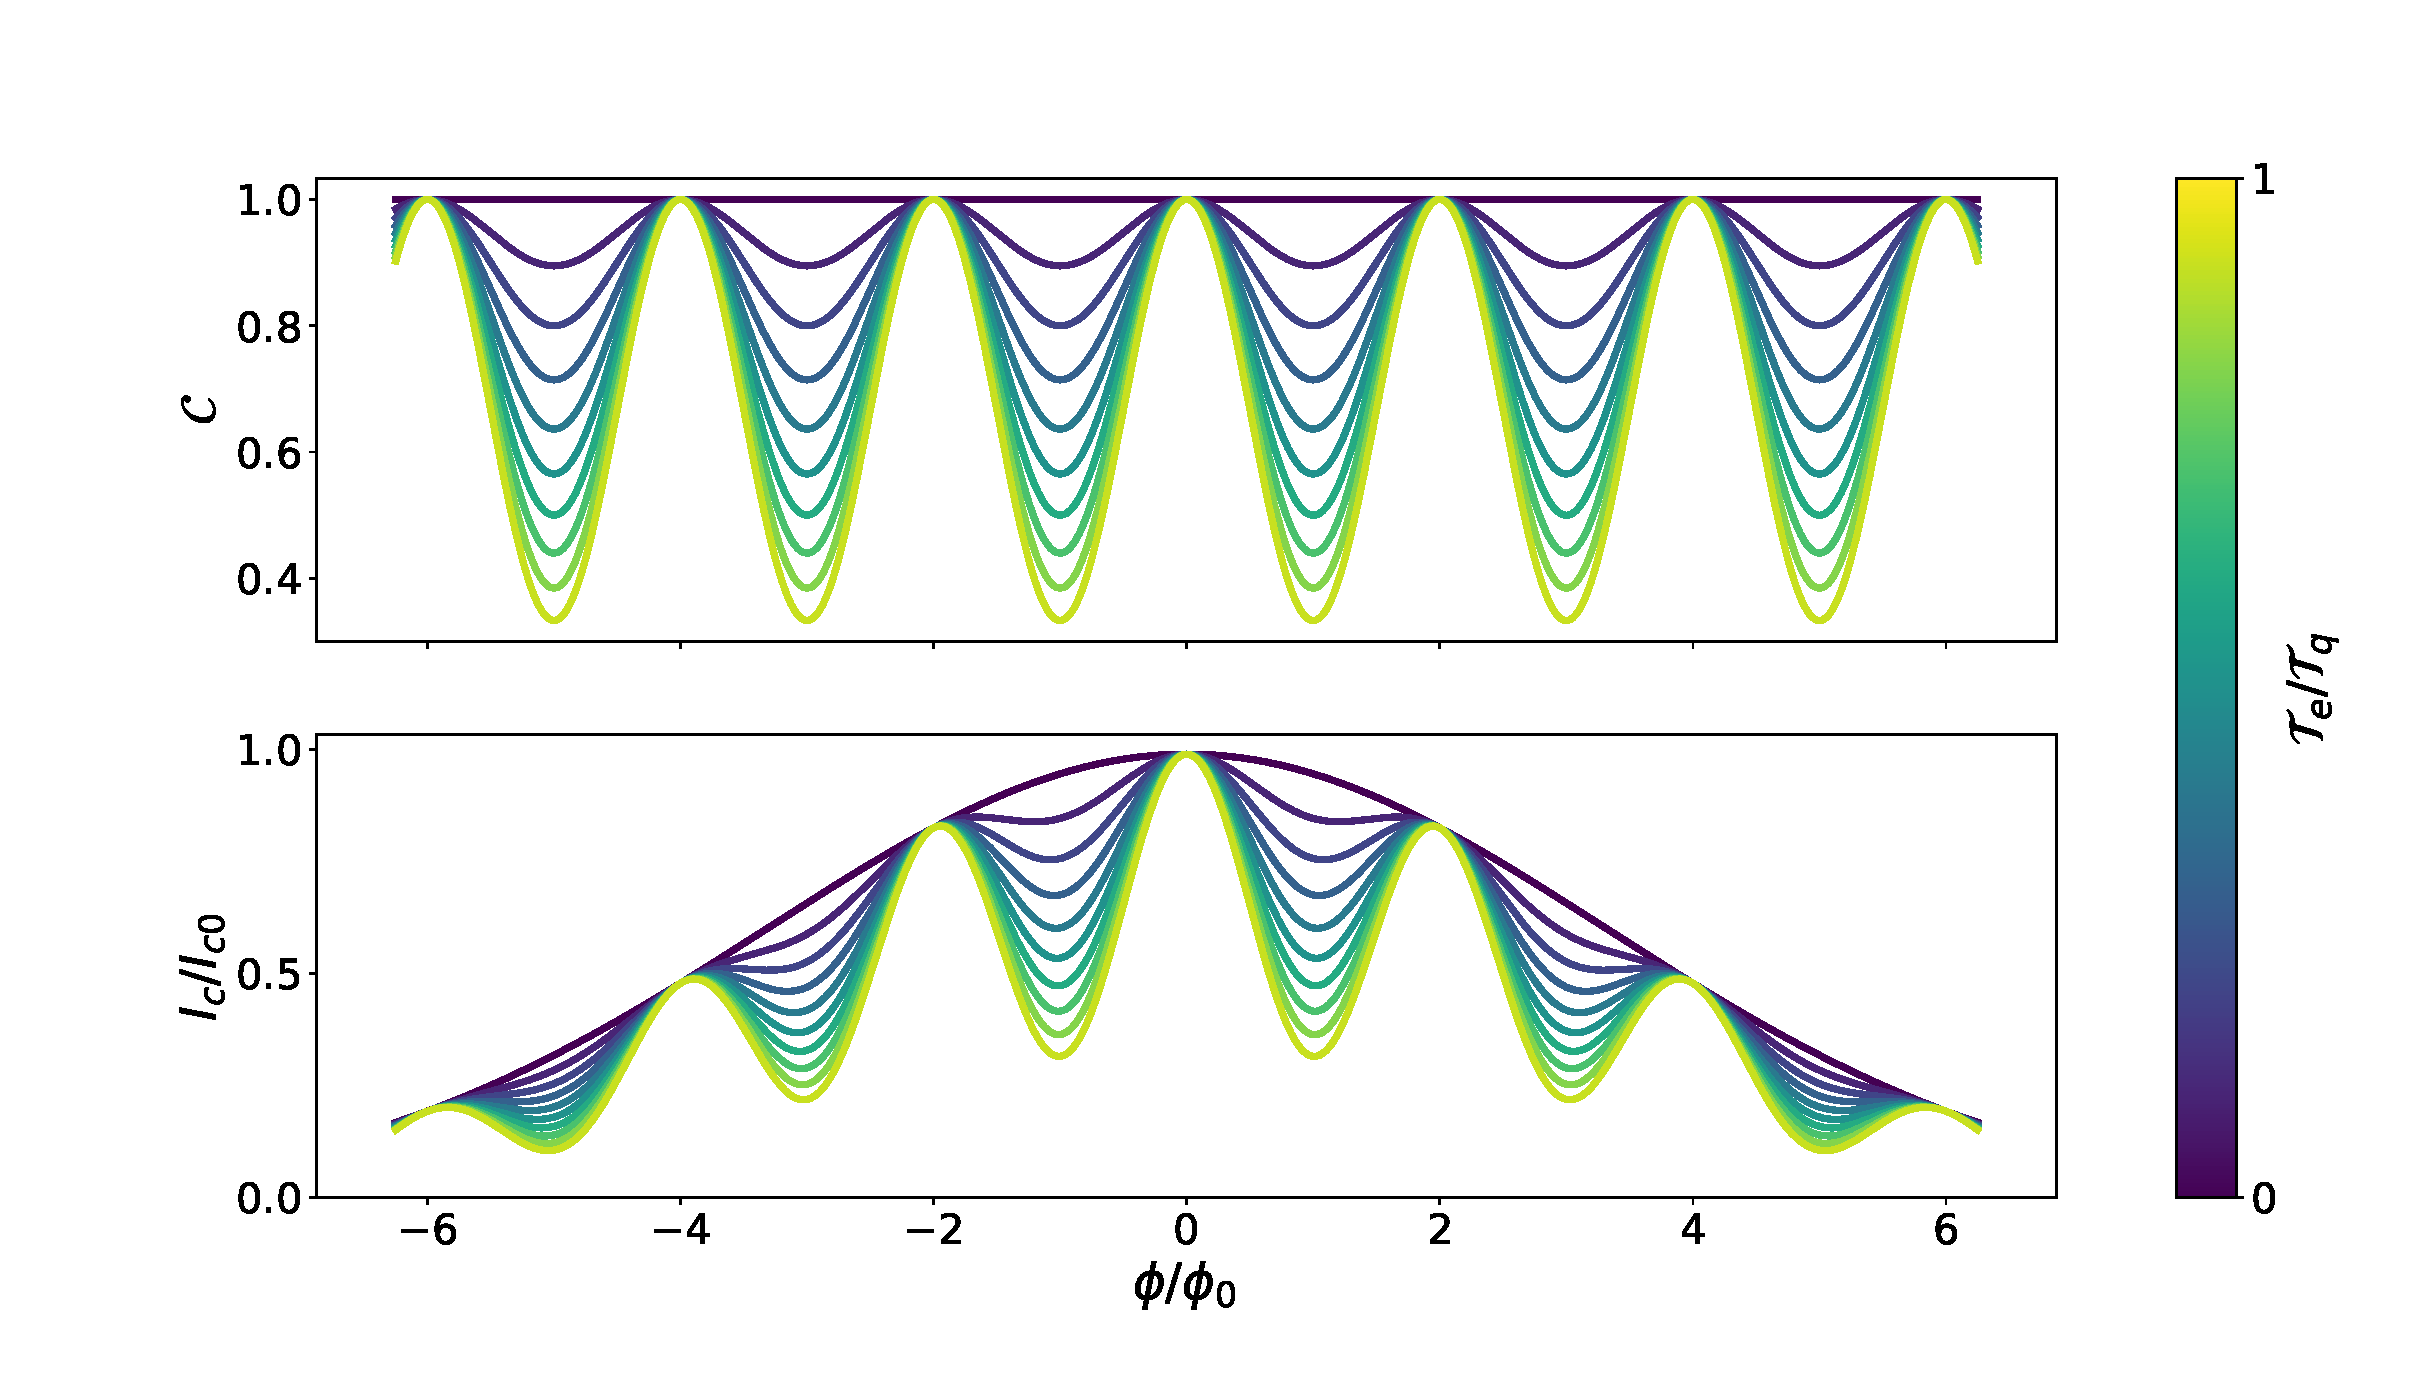
\includegraphics[width=\textwidth]{figure/analyticalmodel/edge-current-modulation}
\caption{Upper plot: Correction factor $\mathcal{C}$ versus magnetic flux $\phi / \phi_0$ for different values of $\mathcal{T}_e / \mathcal{T}_q$. Lower plot: critical current for the QPC from eq. (\ref{eq:qpc-integral}), modulated by $\mathcal{C}$.}\label{fig:edge-current-modulation}
\end{figure}

In figure \ref{fig:edge-current-modulation} visualizes, how the total critical current is affected if edge channels are present. The color scale indicates the ratio of transmissions coefficients $\mathcal{T}_e$ and $\mathcal{T}_q$. When $\mathcal{T}_e / \mathcal{T}_q \approx 1$, meaning the transmission of the edges is as strong as the transmission of the QPC, the current is strongly modulated and the bell-shaped pattern is destroyed. When the ratio is small, the Gaussian curve is not affected by the modulation.
The data presented in chapter \ref{ch:experiment} in section \ref{sec:experiment-superconducting} suggests that edge current do not have a major influence in this setup. 

\section{Barrier With Finite Split Width: Transition To The QPC Set-up}
\begin{figure}
\centering
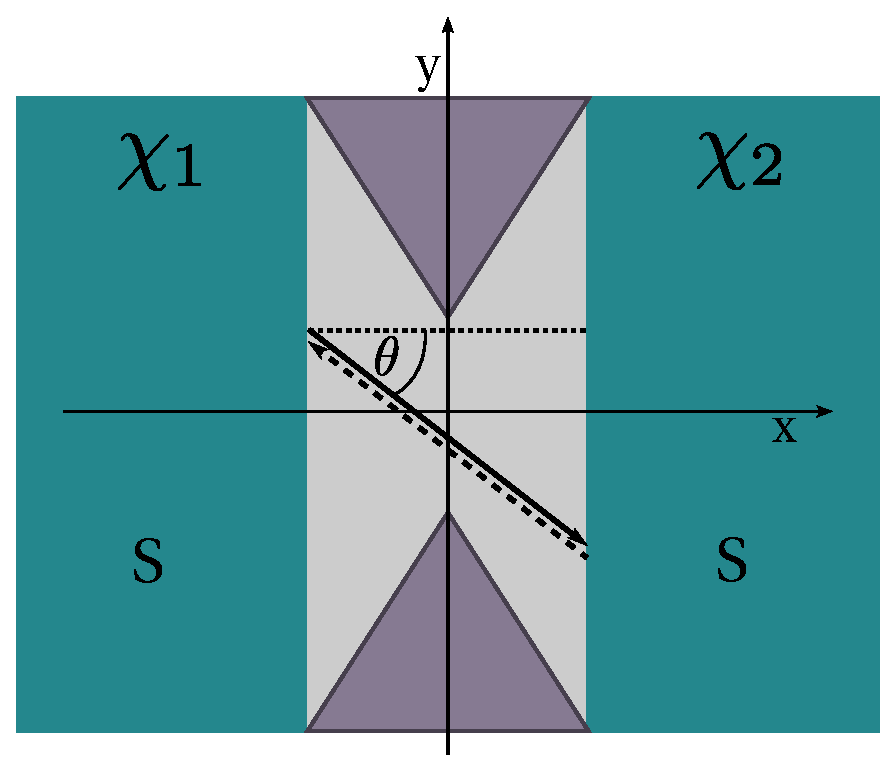
\includegraphics[width=0.6\textwidth]{figure/analyticalmodel/hourglass_csch}
\caption{An SNS junction with hourglass-shaped constriction on top. The split is located at $(x, y) = (0, \pm w_s / 2)$ and  the trajectory is parametrized by the angle $\theta$. }\label{fig:hourglass}
\end{figure}
The QPC set-up and the SNS set-up without barriers can be linked conceptually by investigating an hourglass-shaped set-up. This set-up constricts the trajectories through a split with a finite width $w_s$ as visualized in figure (\ref{fig:hourglass}). When considering only straight trajectories, this split width models the transition to the QPC in the limit of $w_s \rightarrow 0 $. The difference to the QPC is simply the parametrization of the angles: with a finite $w_s$, trajectories are parametrized by only one angle $\theta$, the direction does not change after passing the split:
\begin{equation}
J \left( \chi, \phi \right) = \frac{2 e v_F}{\pi \lambda_F L^2} \int_{-W/2}^{W/2} d y_1 \int_{\theta_\text{min}}^{\theta_\text{max}} \frac{\mathcal{J}(\tilde{\chi} ( y_1, y_2 ) )}{\left( 1 + \left(\frac{y_2 - y_1}{L}\right)^2 \right)^2},
\end{equation}
where
\begin{eqnarray}
\theta_\text{min} &=& \arctan\left( -\frac{w_s + 2y_1}{L} \right),\\
\theta_\text{max} &=& \arctan\left( \frac{w_s - 2y_1}{L} \right).
\end{eqnarray}
When $w_s$ is small enough, like in the QPC case, two independent trajectories are considered with two parametrization angles $\theta_1$ and $\theta_2$. 
%TODO size of $w_s$?
This set-up is particularly interesting because the impact of asymmetry in the junction can be studied. When relocating the split by for example moving it along the $x$-axis, the possible trajectories are limited. As a consequence, the Fraunhofer pattern changes. 
%TODO cite?